
\begin{concept}[15cm]
\textit{Nội dung chương này sẽ tập trung trình bày những kiến thức cần thiết cho quá trình thực hiện đề tài; từ những kiến thức phải nắm được về hệ thống BE-PUM do đây là một đề tài làm việc dựa trên đó; và mỗi khi làm việc với một thư viện bất kỳ, đòi hỏi ta phải tìm hiểu cách thức làm việc với thư viện đó và cả những kiến thức cần thiết do bộ thư viện ấy yêu cầu. Đồng thời cũng trình bày các kiến thức cơ bản về hợp ngữ assembly, từ đó có cái nhìn tổng quan về assembly để tiến hành xây dựng chương trình BE-PUM.}
\end{concept}

\section{Làm việc với BE-PUM}

Trong BE-PUM có xây dựng một hệ thống mô tả môi trường làm việc tương tự như trên một hệ thống máy tính khởi chạy ngoài thực tế; chúng bao gồm các thành phần chính mà đề tài sẽ ảnh hưởng đến như sau:

\begin{itemize}
\item 	\textbf{Chồng (stack)} là một đơn vị dùng để lưu trữ giá trị theo nguyên tắc xếp chồng lên nhau, hoạt động theo nguyên lý vào sau ra trước (Last In First Out (LIFO)). Nó được dùng với nhiều mục đích khác nhau, ví dụ như để ghi nhận địa chỉ cần trở về khi thực hiện gọi một chương trình con, hay để ghi nhận các giá trị của các tham số truyền vào khi gọi một hàm Windows API.\\

\item 	\textbf{Bộ nhớ (memory)} dùng để lưu trữ toàn bộ giá trị của các vùng nhớ mà chương trình đang làm việc. Windows API cũng có khả năng tương tác với phần này; do vậy, đòi hỏi khi xây dựng xử lý API cần đảm bảo kết quả chính xác cho thành phần này.\\

\item 	\textbf{Thanh ghi (register)} là một vùng nhớ có dung lượng nhỏ nhưng lại có khả năng truy xuất rất nhanh, chúng được dùng để làm vùng nhớ tạm, trung gian cho các câu lệnh chạy trong hệ thống. Mỗi khi gọi một hàm bất kỳ, nếu như kiểu trả về khác void thì giá trị trả về sẽ được lưu trữ vào thanh ghi EAX.\\
\end{itemize}


\section{Các câu lệnh hợp ngữ}

	\subsection{Assembly}
	
		\subsubsection{Bộ nhớ assembly}	
		 Biến và hằng trong assembly có tính chất và mục đích sử dụng khác nhau. Thông qua các câu lệnh liên kết chặn chẽ với bộ nhớ là các thanh ghi bộ nhớ, trạng thai, các cờ được đánh dấu mà thông qua đó để thực thi chương trình.\\

		Các thanh ghi bộ nhớ:		
		\begin{center}
			\begin{figure}[htp]
				\begin{center}
					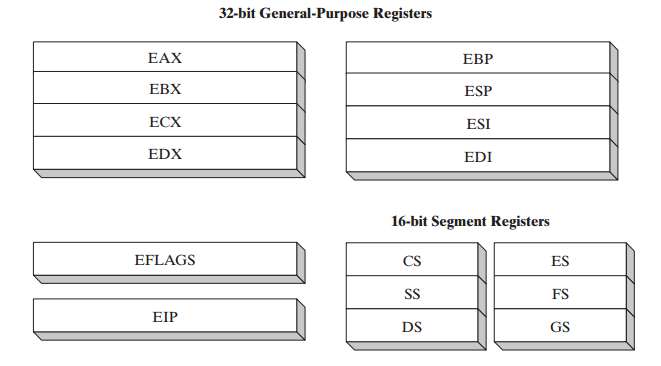
\includegraphics[scale=0.5]{ThanhGhi.png}
				\end{center}
				\caption{Các thanh ghi \protect\footnotemark}
				\label{fig:Flow}
			\end{figure}
			\footnotetext{ Trích dẫn hình ảnh trong sách Assembly Language}
		\end{center}
		
		Trong đó các thanh ghi General-Purpose gồm những thanh ghi có số bit nhỏ hơn:	
		\begin{center}
			\begin{figure}[htp]
				\begin{center}
					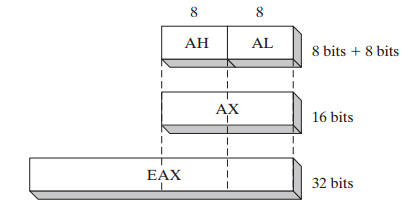
\includegraphics[scale=0.5]{ThanhGhi32bit.png}
				\end{center}
				\caption{ Các thanh ghi \protect\footnotemark}
				\label{fig:Flow}
			\end{figure}
			\footnotetext{Trích dẫn hình ảnh trong sách Assembly Language}
		\end{center}
		
		Ví dụ: thanh ghi EAX(32 bit địa chỉ) có thể được chia ra gồm thanh ghi AX(16 bit địa chỉ). Thanh ghi AX tiếp tục chia địa chỉ thành AH(8 bit) và AL(8 bit). Việc chia địa chỉ như thế giúp tối ưu bộ nhớ khi sử dụng.
		\begin{longtable}{ | m{3cm} | m{3cm} | m{3cm}  | m{3cm}| }
			\hline
				32 Bit & 16 Bit & 8Bit & 8 Bit\\
			\hline
			\hline
				EAX & AX	& AH	 & AL\\
			\hline			
				EBX & BX	& BH	 & BL\\
			\hline		
				ECX & CX	& CH	 & CL\\		
			\hline
				EDX & DX	& DH	 & DL\\
			\hline
			\caption{Bảng chia bộ nhớ 32-bit, 16-bit, 8-bit}
			\label{table:tbthanhghi}
		\end{longtable}
		
			Đối với một số thanh ghi có 32-bit địa chỉ có thể chia ra 16-bit địa chỉ, không thể chia nhỏ hơn. Bảng chi bộ nhơ thanh ghi có thể chia ra 16-bit địa chỉ.\\
			\begin{longtable}{ | m{3cm} | m{3cm} | }
			\hline
				32 Bit & 16 Bit\\
			\hline
			\hline
				ESI & SI\\
			\hline			
				EDI & DI\\
			\hline		
				EBP & BP\\		
			\hline
				ESX & SP\\
			\hline
			\caption{Bảng chia bộ nhớ 32-bit,16-bit}
			\label{table:tbthanhghi}
		\end{longtable}
		
	Mỗi thanh ghi có một chức năng khác nhau: 
\begin{itemize}
	\renewcommand{\labelitemi}{\textbullet}
	\item	EAX: thường được sử dụng trong các phép tính số học: cộng, trừ, nhân, chia, các phép toán logic, chuyển dữ liệu.
	\item EBX: được sử dụng như thanh ghi địa chỉ .
\item	ECX: được sử dụng trong các phép lặp, chuyển bit địa chỉ, xoay bit địa chỉ.
\item	EDX: thường được dùng để lưu dữ liệu, kết hợp vơi thanh ghi EAX thực hiện các phép toán nhân, cộng.
\item	ESP: luôn trỏ thới địa chỉ đỉnh stack hiện thời.
\item	EBP: thanh ghi dùng để truy cập giá trị, nhập dữ liệu stack. Khác với thanh ghi ESP, thanh ghi EBP còn được sử dụng để truy cập trong các đoạn chương trình khác nhau.
\item	EIP: thanh ghi con trỏ chỉ dẫn, giá trị của thanh ghi không thể thay đổi một các trực tiếp, chỉ thay đổi khi trỏ tới câu lệnh tiếp theo. Thanh ghi EIP lưu giá trị trỏ tơi của câu lệnh tiếp theo sẽ được gọi. 
\item	ESI, EDI: thanh ghi chỉ số nguồn và chỉ số đích thường được dùng trong các thao tác, xử lý mảng và chuỗi.
\end{itemize}	
	
	Thanh ghi EFLAGS bao gồm các chuỗi nhị phân được điều khiển bởi CPU hoặc phản ánh một số phép toán của CPU. Trạng thái của CPU. Bao gồm 8 cờ hiệu với mỗi loại cờ có chức năng khác nhau:
\begin{itemize}
	\renewcommand{\labelitemi}{\textbullet}		
		\item CF(Carry Flag cờ nhớ): cờ được bật khi phép tính có nhớ bit.
		\item ZF(Zero Flag cờ 0): cờ được bật khi phép tính vừa thực hiện là 0.
\item SF(Sign Flag cờ dấu): cờ này được bật khi kết quả thực phép tính có bit dấu.
\item	OF(Overflow Flag cờ tràn): cờ được bật khi kết quả thực hiện phép tính bị tràn số học.
\item	PF(Parity Flag cờ chẵn lẽ): cờ được bật khi kết quả của phép tính có chẵn bit 1.
\item	AF(Auxilary Flag cờ nhớ phụ): cờ được bật khi phép tính được thực hiện có sử dụng bit nhớ phụ.
\item IF(Interrupt Flag cờ ngắt): cờ được bật khi có thông báo cho phép ngắt xảy ra.
\item DF(Direction Flag cờ hướng): cờ được bật và sử dụng khi thao tác với mảng và chuỗi, sử dụng để giảm chỉ số tự động thi thao tác.
\end{itemize}	

		\subsubsection{Câu lệnh assembly}
		Một câu lệnh assembly có cú pháp đầy đủ như sau: 
		 \begin{center}		 
			\fontshape{it}  
			\selectfont
		 	$[ $ Nhãn lệnh: $]$  	$<$ Tên lệnh $<$ 	$[$ Các toán hạng $]$	$[$ ;lời chú thích $]$ \\
		 \end{center}			
		Trong đó:
		
		\begin{itemize}
		\renewcommand{\labelitemi}{\textbullet}		
		\item $[$ Nhãn lệnh: $]$  là một chuỗi ký tự kết thúc bằng dâu “:”, được thanh thế cho địa chỉ câu lệnh, được sử dụng trong câu lệnh If, else hoặc cần gọi thay bằng địa chỉ câu lệnh. Trong một chương trình không thể có hai nhãn lệnh trùng tên, tên nhãn lệnh không được trùng với tên thủ tục.
		\item $<$Tên lệnh $>$là một trong số những lệnh gợi nhớ của mã assembly, không phân biệt chữ hoa, chữ thường. Mỗi dòng lệnh chỉ đảm nhận một câu lệnh, mỗi câu lệnh phải được đặt trên một dòng.
		\item $[$Các toán hạng$]$ là các đối tượng mà câu lệnh sẽ tác động vào. Tùy theo từng câu lênh mà có 0 toán hạng, 1 toán hạng, 2 toán hạng, 3 toán hạng. Toán hạng đầu tiên gọi là toán hạng đích, toán hạng thứ 2 gọi là toán hạng nguồn. Với câu lệnh có 3 toán hạng thì chỉ có 1 toán hạng đích trong câu lệnh đó. 
		\item $[$; lời giải thích$]$ khi biên dịch thì lời giải thích không được biên dịch sang mã máy, chỉ có tác dụng với người đọc chương trình. Giúp người đọc dễ hiểu các câu lệnh.
		\end{itemize}

	Ví dụ 1: xét câu lệnh sau đây: 
	 \begin{center}		 
		VD1: mov ax, bx	;lưu giá trị thanh ghi ax từ thanh ghi bx
	\end{center}
	Trong đó:
	\begin{itemize}
		\renewcommand{\labelitemi}{\textbullet}			
	  \item	VD1 : là chuỗi ký tự nhãn lệnh.
	\item	mov: tên lệnh với chức năng lưu giá trị đích(ax) từ giá trị nguồn (bx).
	\item	ax, bx: các toán hạng, trong trường hợp này là các thanh ghi bộ nhớ 16 bit.
	\item $;$ lưu giá trị thanh ghi ax từ thanh ghi bx : lời giải thích, chú thích thêm.
	\end{itemize}
	
	Xem các câu lệnh sau đây:
	\begin{itemize}
	\renewcommand{\labelitemi}{\textbullet}		
	\item  NOT	: đây là câu lệnh không có toán hạng.
	\item	Mov ax, bh: câu lệnh này có 2 toán hạng ax (toán hạng đích) thanh ghi 16 bit, bh (toán hạng nguồn) thanh ghi 8 bit.
	\item	Add ah, sqt: câu lệnh này có 2 toán hạng ah (toán hạng đích) thanh ghi 8 bit, sqt (toán hạng nguồn) một biến được gán trước có kiểu dữ liệu là byte.
	\item	Mov ax, [SI]: câu lệnh này có 2 toán hạng ax (toán hạng đích) thanh ghi 16 bit, [SI] (toán hạng nguồn) là một ô nhớ.
	\item	Imul ax, bx, 10: câu lệnh này có 3 toán hạng ax (toán hạng đích) thanh ghi 16 bit, bx (toán hạng nguồn) thanh ghi 16 bit, và một hằng số (10).
	\end{itemize}

	Câu lệnh Imul có tới 3 toán hạng, toán hạng đích (ax) sẽ được lưu kết quả của phép nhân từ toán hạng nguồn (bx) nhân với hằng số (10: tức toán hạng thứ 3).\\
	Bảng ký hiệu toán hạng:
	\begin{longtable}{ | m{3cm} | m{12cm} | }
			\hline
				Toán hạng & 16 Mô tả\\
			\hline
			\hline
				reg8 & Thanh ghi có 8 bit địa chỉ: AH, AL, BH, BL, CH, CL, DH, DL \\
			\hline			
				reg16& Thanh ghi có 16 bit địa chỉ: AX, BX, CX, DX, SI, DI, SP, BP\\
			\hline		
				reg32& Thanh ghi có 32 bit địa chỉ: EAX, EBX, ECX, EDX, ESI, EDI, ESP, EB\\
			\hline	
				reg&	Bất kỳ thanh ghi nào\\
			\hline	
				sreg & Thanh ghi segment có 16 bit địa chỉ: CS, DS, SS, ES, FS, GS\\
			\hline	
				imm	&8- , 16-, hoặc 32- bit giá trị được truyền vào\\
			\hline	
				imm8	& Giá trị hằng số truyền vào kiểu byte 8-bit\\
			\hline	
				imm16	& Giá trị hằng số truyền vào kiểu word 16-bit\\
			\hline	
				imm32&	Giá trị hằng số truyền vào kiểu doubleword 32-bit\\
			\hline	
				reg/mem8& Toán hạng 8 bit, có thể là thanh ghi có 8-bit địa chỉ hoặc bộ nhớ byte\\
			\hline	
				reg/mem16&	Toán hạng 16 bit, có thể là thanh ghi có 16-bit địa chỉ hoặc bộ nhớ word\\
			\hline	
				reg/mem32	& Toán hạng 32 bit, có thể là thanh ghi có 32-bit địa chỉ hoặc bộ nhớ doubleword\\
			\hline	
				mem	& Bất kỳ bộ nhớ 8-, 16-, 32- bit\\
		\hline	
			\caption{Bảng ký hiệu toán hạng:}
			\label{table:tbkyhieu}
	\end{longtable}
	
		Phân tích câu lệnh mov: \\
		Cú pháp: 
		\begin{itemize}
			\renewcommand{\labelitemi}{\textbullet}	
			\item Mov [toán hạng đích], [toán hạng nguồn].
			\item	Mov reg/mem8, reg8
			\item Mov reg/mem16, reg16
			\item	Mov reg/mem32, reg32
			\item	Mov reg8, reg/mem8
			\item	Mov reg16, reg/mem16
			\item	Mov reg32, reg/mem32
			\item	Mov reg/mem16, sreg
			\item	Mov sreg, reg/mem16
			\item	Mov reg8, imm8
			\item	Mov reg16, imm16
			\item	Mov reg32, imm32
			\item	Mov reg/mem8, imm8
			\item	Mov reg/mem16, imm16
			\item	Mov reg/mem32, imm32	
		\end{itemize}
	
	Trong đó: 
	\begin{itemize}
		\renewcommand{\labelitemi}{\textbullet}	
			\item  $[$ Toán hạng đich$]$: có thể là thanh ghi (8 bit, 16 bit, 32 bit), ô nhớ (địa chỉ của ô nhớ) hay một biến nào đó.$[$Toán hạng đích$]$không thể là hằng số.
			\item $[$ Toán hạng nguồn $]$: có thể là hằng số, biến, thanh ghi, ô nhớ.
	\end{itemize}

	Xem ví dụ sau:
		\begin{itemize}
		\renewcommand{\labelitemi}{\textbullet}	
		\item	Mov ax, bx 		; đặt giá trị của thanh ghi bx vào ax.
		\item Mov ax, 5		; đặt giá trị 5 vào thanh ghi ax.
		\item	Mov bx, 5*3 		; đặt giá trị 5*3 vào thanh ghi bx.
		\item Mov DI, ‘A’		; đặt mã ASCII của ‘A’ vào thanh ghi DI
		\item Mov ch, var		; đặt giá trị của biến var kiểu byte vào thanh ghi ch.
		\item	Mov bh, 300		; giá trị không hợp lệ vì bh có kiểu byte giới hạn 255 nên không thể gán giá trị 300 vào bh.
		\item	Mov ch, ax		; giá trị không hợp lệ vì giá trị thanh ghi ax (16 bit) không thể gán giá trị vào thanh ghi ch (16 bit).  
		\end{itemize}

		\subsubsection{Tập giá trị}
		Khác với các ngôn ngữ lập trình khác, kiểu giá trị của assembly có đôi chút khác biệt, được tính theo bit, tùy theo yêu cầu sử dụng của người lập trình. \\
		Các kiểu dữ liệu:
		\begin{longtable}{ | m{3cm} | m{8cm} | }
			\hline
				Kiểu & Cách sử dụng\\
			\hline
			\hline
				BYTE & 	kiểu số nguyên 8-bit không dấu.\\
			\hline
				SBYTE	& kiểu số nguyên 8-bit có dấu.\\
			\hline
				WORD& 	kiểu số nguyên 16-bit không dấu.\\
			\hline
				SWORD	& kiểu số nguyên 16-bit có dấu.\\
			\hline
				DWORD& 	kiểu số nguyên 32-bit không dấu.\\
			\hline
				SDWORD& 	kiểu số nguyên 32-bit có dấu.\\
			\hline
				FWORD	& kiểu số nguyên 48-bit.\\
			\hline
				QWORD& 	kiểu số nguyên 64-bit\\
			\hline
				TBYTE& 	kiểu số nguyên 80-bit (10-byte).\\
			\hline
				REAL4& 	kiểu số thực 32-bit (4-byte) chuẩn IEEE.\\
			\hline
				REAL8& 	kiểu số thực 64-bit (8-byte) chuẩn IEEE.\\
			\hline
				REAL10& 	kiểu số thực 80-bit (10-byte) chuẩn IEEE.\\			
			\hline
					\caption{Bảng kiểu dữ liệu:}
					\label{table:tbkieudulieu}
		\end{longtable}
		
		Ngoài ra còn có một số ký hiệu kiểu số tự nhiên.
		\begin{longtable}{ | m{3cm} | m{6cm} | }
			\hline
				Kiểu & Cách sử dụng\\
			\hline
			\hline
				DB &	kiểu số nguyên 8-bit.\\
			\hline
				DW &	kiểu số nguyên 16-bit.\\
			\hline			
				DD &	kiểu số nguyên hoặc số thực 32-bit.\\
			\hline
				DQ	 &kiểu số nguyên hoặc số thực 64-bit.\\
			\hline
				DT	 &định nghĩa kiểu số nguyên 80-bit (10 byte).\\
			\hline
					\caption{Bảng ký hiệu kiểu số tự nhiên:}
					\label{table:tbkieudulieutn}
		\end{longtable}
		
		Trên cở sở các đơn vị dữ liệu được lưu trên kiến trúc X86, một byte tưng ứng với 8-bit, tưng tự word tưng ứng với 16-bit (2 byte), doubleword tưng ứng với 32-bit (4 byte), quadword tưng ứng với 64-bit (8 byte). Từ đó ta tính toán được phạm vi giới hạn số học của các kiểu số nguyên không dấu và có dấu: 
			\begin{longtable}{ | m{5cm} | m{6cm} | m{3cm} |}
			\hline
				Kiểu lưu trữ &	Phạm vi (từ thấp đến cao)&	Dung lượng\\
			\hline
			\hline
				Byte không dấu &	0 đến 255&	1 byte\\
			\hline
				Word không dấu	&0 đến 65,535&	2 bytes\\
			\hline
				Double word không dấu	 &0 đến 4,294,967,295&	4 bytes\\
			\hline
				Quadword không dấu	&0 đến 18,446,744,073,709,551,615&	8 bytes\\
			\hline
				\caption{Bảng phạm vi kiểu dữ liệu số không dấu}				
			\end{longtable}
		
			\begin{longtable}{ | m{5cm} | m{7cm} |}
			\hline
				Kiểu lưu trữ	& Phạm vi (từ thấp đến cao)\\
			\hline
			\hline
				Byte có dấu	& -128 đến +127\\
			\hline
				Word có dấu &	-32,768 đến +32,767\\
			\hline	
				Double word có dấu &	-2,147,483,648 đến +2,147,483,647\\
			\hline	
				Quadword có dấu	 & -9,223,372,036,854,775,808 đến +9,223,372,036,854,775,807 \\
			\hline
			\caption{Bảng phạm vi kiểu dữ liệu số có dấu}				
			\end{longtable}		
		
		\subsubsection{Kiếu giá trị}
		\subsubsection*{Hằng số}
		Kiểu hằng số nguyên được dùng trong hợp ngữ assembly là một chuỗi số đứng trước nó là dấu của số nguyên đó, tiếp theo là chuỗi số và cuối cùng là cơ số để xác định chuỗi số đó. Cú pháp của chuỗi số:		
		\begin{center}
			\fontshape{it}  
			\selectfont
		 	$[{+|-}]$ chuỗi số$ [$cơ số$]$
		\end{center}
	
	Cơ số là một trong những dạng cơ số dưới đây (không phân biệt chứ hoa hay chữ thường):
		\begin{itemize}
		\renewcommand{\labelitemi}{\textbullet}	
			\item	h	: Hexadecimal hệ cơ số 16
			\item	q/o	: Octal hệ cơ số 8
			\item	d	: Decimal hệ cơ số 10
			\item	b	: Binary hệ cơ số 2
		\end{itemize}			
	Nếu không có ký hiệu cơ số thì mặc định số đó là hệ cơ số 10. Dưới đây là một số ví dụ:
	\begin{itemize}
	\item	26		: 26 hệ cơ số 10
	\item	26d		: 26 hệ cơ số 10
	\item	11010011b	: 11010011 hệ cơ số 2
	\item	42q		: 42 hệ cơ số 8
	\item	42o		: 42 hệ cơ số 8
	\item	1Ah		: 1A hệ cơ số 16
	\end{itemize}	
	
	\subsubsection*{Biểu thức số nguyên}
	Biểu thức số nguyên là các biểu thức toán học mà các toán hạng thuộc kiểu số nguyên. Các biểu thức toán học được xếp theo thứ tự ưu tiên, việc xếp thứ tự này khá quan trọng vì nó ảnh hưởng đến kết quả của một biểu thức. Dưới đây là bảng biểu thức toán học được sắp thứ tự ưu tiên cao nhất là 1 và thấp nhất là 4:	\\
	\begin{longtable}{ | m{3cm} | m{5cm} |m{5cm} |}
			\hline
				Toán tử &	Tên &	Thứ tự ưu tiên\\
			\hline
			\hline
			$()$	 &	Dấu ngoặc&		1\\
			\hline
			$+, -$ &		Dấu dương, âm&		2\\
			\hline
			$*, /$	&	Nhân, chia&		3\\
			\hline
			MOD	&	Chia lấy dư&		3\\
			\hline
			$+,-$	&	Cộng, trừ	&	4\\
			\hline
			\caption{Thứ tự ưu tiên biểu thức toán}
	\end{longtable}
	Xem các ví dụ dưới đây để hiểu rõ hơn:
	\begin{itemize}
	\item  4 $+$ 5 $*$ 3 		: Thực hiện phép nhân trước khi thực hiện phép cộng
	\item	 12 – 2 MOD 3	: Thực hiện phép chia lấy dư trước khi thực hiện phép trừ
	\item	 $-$7 $+$ 2			: Lấy dấu của số 7 trước khi thực hiện phép cộng với 2
	\item	$($5 $+$ 3$) *$ 7		: Thực hiện biểu thức trong ngoặc trước khi thực hiện phép nhân. 
	\end{itemize}
	
	\subsubsection*{Kiểu ký tự và chuỗi}
	Kiểu ký tự và chuỗi ký tự trong hợp ngữ assembly dựa trên bảng mã ASCII để xây dựng. Biến có kiểu ký tự được lưu dưới dạng mã nhị phân của bảng mã ASCII. 
	Cách khai báo biến có kiểu ký tự:
	\begin{itemize}
		\item	‘A’ 
		\item	“b” 
	\end{itemize}
	Một chuỗi ký tự được đặt trong dấu nháy đơn (‘’)  hoặc nháy kép (“”):
	\begin{itemize}		
		 \item  ‘ABCDEF’
		\item	“AAAA”
		\item	“Hom nay la thu hai”
		\item	‘123456’ 
	\end{itemize}	
		
		\subsubsection{Cấu trúc một chương trình assembly}
			Hiện này, hầu hết các hệ điều hành hiện nay, đặc biệt là hệ điều hành Microsoft đều hỗ trợ hai dạng cấu trúc tập tin thực thi là COM và EXE. Nhưng trong BE-PUM tập trung phân tích cấu trúc tập tin EXE. Cấu trúc tập tin EXE và COM có sự khác biệt rất lớn. Cấu trúc tập tin EXE được chia thành ba đoạn: Mã lệnh (Code), dữ liệu (Data), ngăn xếp (Stack). Trong khi đó cấu trúc tập tin COM chỉ có một đoạn mã lệnh được gom từ ba đoạn trong cấu trúc tập tin EXE. \\

Ngoài ra, cấu trúc tập tin EXE có thể bố trí hơn ba đoạn bộ nhớ. Do đó, khi thiết kế chương trình, hay gặp phải chương trình được bố trí hơn ba đoạn thì cần phải quan tâm đến các modun của chương trình, sự liên kết giữa các đoạn với nhau. \\

Cấu trúc chương trình được giới thiệu, phân tích dưới đây là cấu trúc tập tin thực thi EXE, nêu lên những khái niệm cơ bản của một chương trình assembly. \\
	\begin{normalsize}
			\setlength{\parindent}{1cm}		
			\renewcommand{\rmdefault}{cmss}
			\textit {$.$ Model	$<$ chế độ bộ nhớ $>$	}		\\	
			\indent  \textit{.Stack 100h } \\			
			\indent \textit{<khai báo dữ liệu>} \\			
			\indent \textit{.Code}\\
			\indent \textit{<Thủ tục chính > PROC}\\ \\
			\indent \textit{<các câu lệnh của chương trình>}\\ \\
			\indent \textit{< Thủ tục chính> } \\
			\indent \textit{Endp}\\
			\indent \textit{<Các thủ tục khác được khai>}\\
			\indent \textit{END}\\
	\end{normalsize}
	
	Trong cấu trúc được đưa ra, các từ \textit {.Model, .Stack, .Data, .Code, PROC, Endp, END} là các từ để hướng dẫn thực thi một chương trình assembly. \\

Nhìn vào cấu trúc chương trình, ta thấy rõ một chương trình assembly được phân tích ra gồm 3 đoạn chính: đoạn \textit{Code}, chứa toàn bộ mã lệnh, nơi thực thi của chương trình, đoạn \textit{Data} nơi chứa các biến dữ liệu được khai báo của chương trình, đoạn Stack nơi chứa stack của chương trinh khi chương trình được nạp vào bộ nhớ để thực thi.\\

Hướng dẫn \textit{.Model} được đạt ngay trên đầu của cấu trúc chương trình nhằm mục đích khai báo chế độ nhớ mà chương trình sử dụng để thực thi.\\

Hướng dẫn \textit{.Stack} đặt ở đầu chương trình mục đích để khai báo kích thước stack được sử dụng để thực thi chương trình. Kích thước stack thường được khai báo là 100h (256) byte.\\

Ví dụ chương trình được viết theo cấu trúc EXE:\\

\begin{boxedminipage}{15cm}
	\begin{normalsize}						
				\textit {.model small}
				\begin{changemargin}{1cm}{0.5cm} 
     			\textit { include \textbackslash masm32 \textbackslash include \textbackslash windows.inc}  \\  
				\textit { include \textbackslash masm32 \textbackslash include \textbackslash windows.inc} \\
				\textit { include \textbackslash masm32 \textbackslash include \textbackslash windows.inc} \\
				\textit { include \textbackslash masm32 \textbackslash include \textbackslash windows.inc} \\ \\
				\textit { include \textbackslash masm32 \textbackslash include \textbackslash windows.inc} \\ 
				\textit { include \textbackslash masm32 \textbackslash include \textbackslash windows.inc} \\
				\textit { include \textbackslash masm32 \textbackslash include \textbackslash windows.inc} \\
				\textit { include \textbackslash masm32 \textbackslash include \textbackslash windows.inc} \\
				\textit {stack 100h}
				\end{changemargin}				
				\textit {.data}
				\begin{changemargin}{1cm}{0.5cm} 
						\textit {var1 WORD  200}
				\end{changemargin}				
				\textit {.code}\\
				\textit {start: }
					\begin{changemargin}{1cm}{0.5cm} 
    							\textit {main proc}
    								\begin{changemargin}{1.5cm}{0.5cm} 
        								\textit {mov ax, 775}\\
       							 		\textit {aad   }\\
        								\textit {	mov eax, 100 }\\
       									\textit { aad}\\
        								\textit {	mov bl, 5}\\
        								\textit {	div bl   }\\
										\textit {mov eax, 10}\\
   										\textit {bsf eax, var1}		\\
		  								\textit {ret}
		  							\end{changemargin}	
     						\textit {main endp}
     				\end{changemargin}				
				\textit {end start}
	\end{normalsize}
	\end{boxedminipage}
	
		Ở phần đầu chương trình có khai báo các đường dẫn thư viện hỗ trợ chương trình bằng cú pháp:
		\begin{center}
			\textit { include <đường dẫn>} \\
		\end{center}
	Có thể thấy đoạn chương trình trên sử dụng chế độ bộ nhớ Small. Khai báo kích thước Stack là 100h byte. Trong phần khai báo dữ liệu Data chỉ khai báo một biến duy nhất là var1 có kiểu dữ liệu là word, giá trị của biến là 200. Trong phần Code, tên thủ tục là main, tên thủ tục có thể được đặt tùy ý.\\


	\subsection{Floating-Point Unit (FPU)}
	Kiên trúc Floating-Point Unit (FPU) của Intel cung cấp hiệu quả cao trong khả năng xử lý floating-point. Kiến trúc FPU hỗ trọ xử lý các số nguyên, số thực và Biniary Coded Decimal (BCD)-số nguyên kiểu dữ liệu, và các floating-point được sử lý bằng thuật toán được định nghĩa theo tiêu chuẩn IEEE 754 và 854. Các câu lệnh FPU được thực hiện từ bộ vi sử lý của các dòng lệnh bình thường và được cải thiện đáng kể hiệu quả của các bộ vi xử lý Intel trong xử lý các phép tính có độ chính xác cao, các hoạt động xử lý dấu chấm động.\\
		\subsubsection{Số thực và định dạng Floating-point}	
		Phần này sẽ mô tả cách các số thực được biểu diễn ở dạng dấu chấm động của FPU trong kiến trúc Intel. Đồng thời giới thiệu các thuật ngữ như số normalized, số denormalized, số mũ, số không, và NaN (not a number). 
		
		\subsubsection*{Hệ thống số thực}
		Như thể hiện trong hình 3, hệ thống số thực bao gồm sự liên tục của các số thực từ trừ vô cực (-$\mathbb{\infty}$)  đến cộng vô cực (+$\mathbb{\infty}$) .\\
		\begin{center}
			\begin{figure}[htp]
				\begin{center}
					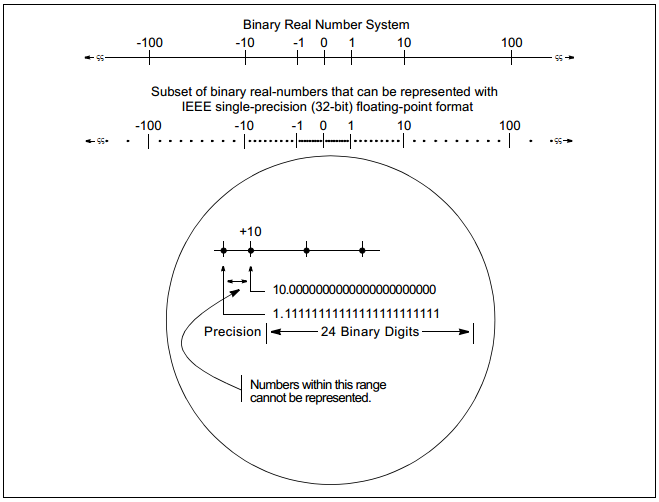
\includegraphics[scale=0.8]{MaNhiPhan.png}
				\end{center}
				\caption{Hệ thống mã nhị phân biểu diễn số thực}				
			\end{figure}
		\end{center}		
		
		Bởi vì kích thước và số lượng thanh ghi của bất kỳ máy tính nào có thể có hạn chế, chỉ có một đoạn mã nhị phân của số thực có thể được sử dụng trong tính toán số thực. Hình 3, phần số thực mà FPU hỗ trợ biểu diễn một giá trị xấp xỉ của một số thực. Phạm vi và độ chính xác của các phần mã nhị phân của số thực được biểu diễn theo định dạng FPU sử dụng để hiện thi cho số thực được sử dụng.
		
		\subsubsection*{Định dạng Floating-point}
		Để tăng tốc độ và hiệu quả của các phép tính số thực, các FPU hiện thị đại diện cho một số thực mà được biểu diễn theo định dạng floating-point. Trong định dạng này, một số thực có ba phần: bit dấu, định trị và số mũ. Định dạng này phù hợp với chuẩn IEEE.\\
		\begin{center}
			\begin{figure}[htp]
				\begin{center}
					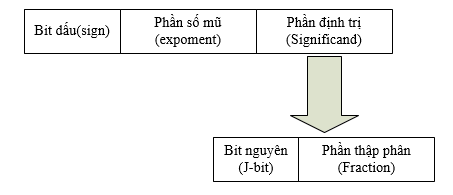
\includegraphics[scale=0.8]{DinhDangMNP.png}
				\end{center}
				\caption{Định dạng mã nhị phân của Floating-point}				
			\end{figure}
		\end{center}		
		
		Bit dấu là một giá trị nhị phân cho biết xem số đó là số âm (1) hay số dương (0). Phần định trị gồm hai phần: bit số nguyên (J-bit) và phần phân số. Phần bit số nguyên thường không được hiện thị, nhưng thay vào đó có giá trị mặc định. Phần số mũ là một số nguyên biểu diễn lũy thừa 2, điều này làm cho phần định trị được tăng lên.
		
		\subsubsection*{Số thông thường (normalized)}	
		Trong hầu hết mọi trường hợp, thanh ghi FPU hiển thị giá trị số thực định dạng thông thường. Ngoại trừ số 0 thì phần định trị luôn được tạo bởi một số thực và theo sau là phần phân số.
		\begin{itemize}
			\item[•	]1.fff…fff
		\end{itemize}
				
	\begin{longtable}{ | m{7cm} | m{7cm} | }
		\hline
				Ký hiệu & Giá trị\\
		\hline
		\hline
			Số thập phân	&178.125\\
		\hline	
			Số thập phân khoa học&	1.78124E102\\
		\hline	
			Số nhị phân khoa học	&1.0110010001E2111\\
		\hline	
			Số nhị phân khoa học (biểu diễn số mũ)	&1.0110010001E210000110\\
		\hline
			Đinh dạng số thực & 0(Bit dấu)  10000110(Phần mũ)	 011001000100000000000001(Phần định trị)\\
		\hline
	\end{longtable}		
		
		Đối với các giá trị thấp hơn 1 thì số 0 ở phia trước được loại bỏ (mỗi số 0 được loại bỏ, số mũ được tăng lên 1).\\

		Để hiện thị số lớn nhất của phần định trị theo định dạng thông thường thì phải cung cấp độ dài của phần định trị này. Để hiện thị số thực theo định dạng thông thường này thì phần định trị sẽ biểu diễn giá trị giữa 1 và 2, phần số mũ sẽ chỉ ra độ tăng của số thực đó.
		
		\subsubsection*{Số mũ (baised expoment)}
			Thanh ghi FPU biểu diễn số mũ theo định dạng cơ bản. Có nghĩa là một hằng số sẽ được thêm vào số mũ được biểu diễn vì vậy số mũ luôn là một số dương. Giá trị hằng số phụ thuộc vào số lượng bit được dùng để biểu diễn số thực trong định dạng dấu chấm phẩy động được sử dụng. Hằng số được chọn sao cho có thể thay đổi giá trị nhưng vẫn không bị tràn số.
			
			\subsubsection*{Số thực và mã hóa phi số thực}
			Có nhiều loại số thực và giá trị đặc biệt có thể được mã hóa theo định dạng dấu phẩy động của FPU:\\
			
			Những số đặc biệt và giá trị đặt biệt được chia thành các loại sau:
			\begin{itemize}
				\renewcommand{\labelitemi}{\textbullet}	
				\item Số 0.
				\item	Số hữu hạn không thông thường (denormalized).
				\item	Số hữu hạn thông thường (normalized).
				\item	Số vô cực
				\item	Không phải là một số (NaNs: Not a number )
				\item	Số không định nghĩa.
			\end{itemize}
			
			Hình ~\ref{fig:SothucNaN} sẽ chỉ rõ cách mã hóa số thực và phi số thực phù hợp với các biểu diễn số thực theo chuẩn IEEE. Ví dụ được sử dụng ở đây miêu tả chuẩn IEEE chính xác đơn (32-bit), các ký hiệu “S” chỉ bit dấu, “E” chỉ số mũ, “F” chỉ phần phân số. ( Giá trị của phần số mũ là một số nguyên). \\

		Các thanh ghi FPU có thể thực hiện các loại and/or trả về đúng giá trị, phụ thuộc vào phép toán được thực hiện. Các phần dưới đây sẽ mô tả các biểu diễn số thực và phi số thực.
		
		\subsubsection*{Số 0}
		Số 0 có thể được biểu diễn là +0 và  -0 phụ thuộc vào bit dấu. Việc mã hóa +0 và -0 tương đương nhau về mặt giá trị. Bít dấu của số 0 phụ thuộc vào phép toán được thực thi và cách thức làm tròn được sử dụng. Bit dấu số 0 có thể xác định tràn số dưới có đang xảy ra hay không, ngoài ra còn xác định bit dấu của giá trị vô cực. 
		
		\subsubsection*{Số normalized và denormalized}
		Trừ số 0, số thực được chia thành 2 dạng: normalized (bình thường) và denormalized (không bình thường). Số normalized bao gồm các giá trị khác 0, có thể mã hóa theo định dạng IEEE trong phạm vi từ số 0 đến vô cực. Trong hình 5, định dạng chính xác đơn với chỉ số mũ từ 0 đến 254 (phạm vi tham số -126 đến 126).
		\begin{center}
			\begin{figure}[htp]
				\begin{center}
					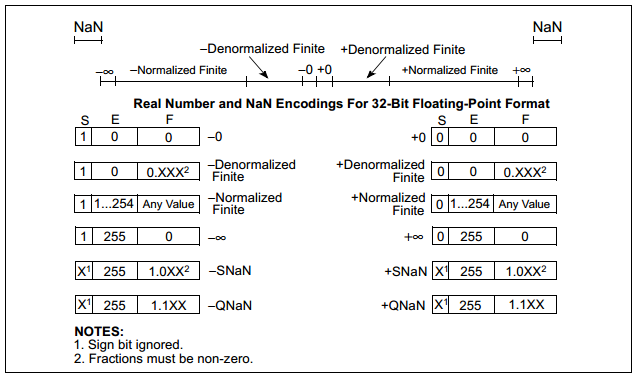
\includegraphics[scale=0.8]{SoThucNaN.png}
				\end{center}
				\caption{Số thực và NaN}				
				\label{fig:SothucNaN}
			\end{figure}
		\end{center}		

	Khi số thực càn gần về số 0, chiều dài bit dùng để biểu diễn số thực không đủ dài để biểu diễn. Bởi vì chỉ số mũ (trong ví dụ này là 32-bit) không đủ lớn để biểu diễn bit dịch phải để loại bỏ các bit 0 ở đầu (xem thêm phụ lục IEEE).\\

	Khi số mũ là số 0, những số nhỏ có thể được biểu diễn bằng những bit số nguyên (và những chuỗi bit ở đầu) của số 0. Số thực trong phạm vi này được gọi là denormalized (hay số rất nhỏ). Việc sử dụng các bit 0 ở đầu cho phép biểu diễn các số rất nhỏ nhưng những số rất nhỏ này là nguyên nhân mất đi sự chính xác (số bit trong phần định trị được giảm đi sẽ được tính toán dựa trên số bit 0 ở phần số mũ).\\

	Khi thực hiện các phép tính trên dấu chấm động, mỗi thanh ghi FPU thực hiện phép toán với số normalized và đưa ra kết quả là một số normalized. Số denormalized biểu diễn cho điều kiện tràn số dưới.\\
	
	Số denormalized được tính bằng kỹ thuật “gradual underflow”. Bảng () sẽ đưa ra một ví dụ của kỹ thuật “gradual underflow” trong xử lý tính toán số denormalized. Ở đây, sử dụng định dạng đơn nên số nhỏ nhất của số mũ là -126. Kết quả trong ví dụ này yêu cầu số mũ là -129. Nếu nhỏ hơn -129 là nằm ngoài phạm vi số mũ cho phép, kết quả của số denormalized bằng cách thêm các bit 0 ở đầu đến khi số mũ nhỏ nhất là -129.\\
		
		\begin{longtable}{ | m{4cm} | m{2cm} |  m{2cm} | m{4cm} | }
			\hline
				Toán hạng & Dấu & Số mũ* & Phần định trị\\
			\hline
			\hline
				Kết quả đúng & 0 & -129 & 1.01011100000..00\\
			\hline
				Số Denormalize & 0 & -128 & 0.10101110000..00\\
			\hline
				Số Denormalize & 0 & -127 & 0.01010111000..00\\
			\hline
				Số Denormalize & 0 & -126 & 0.00101011100..00\\
			\hline
				Kết quả Denormalize & 0 & -126 & 0.00101011100..00\\
			\hline
			\caption{Xử lý số denormalized}
		\end{longtable}
		
	
	Lưu ý: * Số mũ được biểu diễn trong phạm vi (-126 đến 126)\\

	Trong trường hợp tốt nhất, tất cả các bit của phần định trị được dịch phải bằng cách chèm thêm bit 0 ở đầu, tạo ra kết quả là số 0.\\

FPU xử lý với số demormal theo các cách sau đây: 
	\begin{itemize}
			\renewcommand{\labelitemi}{\textbullet}	
			\item	Không được phép tạo số denormalized.
			\item	Cung cấp xử lý ngoại lệ underflow để người lập trình có thể kiểm tra khi số denormalized được tạo ra.
			\item	Cung cấp các toán hạng xử lý số denormalized, cho phép chương trình kiểm tra khi mà các số denormalized được sử dụng như là một toán hạng. 
	\end{itemize}

	Khi một số denormalized ở định dạng chính xác đơn hoặc chính xác kép được sử dụng như một toán hạng, và xử lý ngoại lệ dernormal được đánh dấu, thanh ghi FPU sẽ tự động chuyển giá trị của số denormalized thành normalized bằng cách chuyển sang định dạng mở rộng.

		\subsubsection*{Số vô cực}
		Có 2 số vô cực là âm vô cực và dương vô cực được dùng để biểu diễn số thực âm nhỏ nhất và số thực dương lớn nhất vì vậy có thể biểu diễn dạng dấu chấm động. Số vô cực luôn được biểu diễn bằng bit 0 của phần định trị (phần phân số và bit số nguyên) và số mũ tối đa cho phép của mỗi định dạng (ví dụ: số mũ tối đa 255 đối với định dạng kép).\\

Bit dấu của số vô cực có thể dùng để so sánh. Số vô cực luôn được chỉ định rõ là âm vô cực luôn nhỏ hơn so với bất kỳ số thực cụ thể nào, dương vô cực luôn lớn hơn so với bất kỳ số thực cụ thể nào. Việc tính toán số vô cực luôn chính xác. Ngoại lệ được đánh dấu khi có phép toán xử dụng toán hạng là số vô cực, số vô cực được coi là toán hạng không hợp lệ. \\

Số denormalized biểu diễn cho điều kiện tràn số dưới, 2 số vô cực biểu diễn cho điều kiện tràn số trên. Kết quả số normlized của một phép toán có số mũ nằm trong phạm vi cho phép của số mũ phụ thuộc theo định dạng được sử dụng.
	
		\subsubsection*{NaNs (Not a number: không phải là một số)}
		NaN không phải là một, NaN là phần không nằm trên trục số thực trong hình 5. Việc mã hóa số NaN được chỉ ra trên trục số thực nằm ở cuối và đầu trục số. Khoảng trống này biểu diễn bất kỳ giá trị nào lớn với số mũ tối đa và phần phân số có bit khác không. (Bit dấu được bỏ qua đối với số NaN).\\

	Theo chuẩn IEEE có 2 định dạng cho NaN là: quiet NaNs(QNaNs) và signaling NaNs (SNaNs). Số QnaNs là NaN với phần phân số có hầu hết các bit là 1. Số SNaNs là NaN với phần phân số hầu hết các bit là 0. QNaNs cho phép tạo ra thông qua các phép toán mà không đánh dấu ngoại lệ nào. SNaNs thường thông báo một ngoại lệ không hợp lệ xảy ra khi thực hiện phép toán học. 
	
		\subsubsection*{Số không định nghĩa}
		Đối với mỗi loại dữ liệu của FPU, có một cách để mã hóa giá trị đặc biệt được gọi là giá trị không định nghĩa. Ví dụ, khi tính toán trên trường số thực, số không được định nghĩa là số QNaNs. FPU tạo ra giá trị không định nghĩa khi giá trị được đánh dấu xử lý ngoại lệ.
		
		\subsubsection{Kiến trúc FPU}
		Nhìn tổng quan kiến trúc, FPU là một bộ xử lý các thao tác hoạt động song song với bộ xử lý số nguyên. FPU có các câu lệnh cũng giống như các mã lệnh khác và được thực hiện tuần tự như bộ xử lý số nguyên và chia sẻ đường truyền với bộ xử lý số nguyên. Bộ xử lý FPU, bộ xử lý số nguyên hoạt động độc lập nhau và song song. 
		
		\begin{center}
			\begin{figure}[htp]
				\begin{center}
					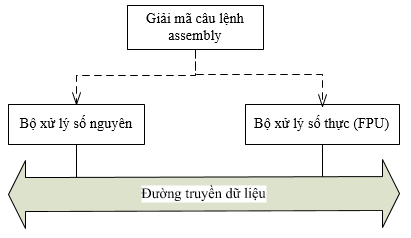
\includegraphics[scale=1.0]{FPUQuanHe.png}
				\end{center}
				\caption{Mối quan hệ giữa bộ xử lý FPU và bộ xử lý Integer}				
				\label{fig:FPUQuanHe}				
			\end{figure}
		\end{center}		
		
		Những câu lệnh được thực thi trong môi trường của FPU hình ~\ref{fig:FPUQuanHe} bao gồm 8 thanh ghi dữ liệu (gọi là thanh ghi dữ liệu FPU) và sau đây là những thanh ghi với mục đích khác:
		\begin{itemize}
			\renewcommand{\labelitemi}{\textbullet}	
			\item	Thanh ghi trạng thái (the status register).
			\item	Thanh ghi điều khiển (the control register).
			\item	Thanh ghi thẻ (the tag word register).
			\item	Thanh ghi con trỏ lệnh (instruction poitnter register).
			\item	Thanh ghi toán hạng (last operand register).
			\item	Thanh ghi Opcode (Opcode register).
		\end{itemize}
		
	Những thanh ghi này được miêu tả trong phần tiếp theo.
	
	\newpage
		\subsection*{Thanh ghi dữ liệu FPU}
	Các thanh ghi dữ liệu FPU (hình ~\ref{fig:MoiTruongFPU}) bao gồm 8 thanh ghi 80-bit. Giá trị được lưu trữ trong các thanh ghi theo định dạng mở rộng. Khi các số thực, số nguyên hoặc giá trị BCD được nén được nạp vào từ bộ nhớ vào trong thanh ghi dữ liệu FPU, các giá trị sẽ tự động chuyển về định dạng mở rộng. Khi tính toán, kết quả được chuyển lại vào bộ nhớ từ bất kỳ thanh ghi FPU, kết quả có thể đã được định dạng mở rộng hoặc được chuyển về định dạng FPU khác (số thực, số nguyên, giá trị BCD được nén).\\

	Những tập lệnh của FPU sẽ xử lý 8 thnh ghi dữ liệu nhưu là một ngăn xếp (stack) các thanh ghi (hình ~\ref{fig:MoiTruongFPU} ) tất cả địa chỉ ác thanh ghi dữ liệu là tương đối so với thanh ghi đỉnh của ngăn xếp. Số lượng thanh ghi ở đỉnh ngăn xếp hiện tại được lưu trữ trong trường TOP (stack TOP) trong thanh ghi trạng thái của FPU. Khi có 1 thao tác nạp thì TOP giảm đi 1 và nạp 1 giá trị vào thanh ghi ở đỉnh mới của ngăn xếp, và thao tác lưu trữ sẽ lưu trữ giá trị thanh ghi từ thanh ghi TOP hiện tại vào bộ nhớ.
		\begin{center}
			\begin{figure}[htp]
				\begin{center}
					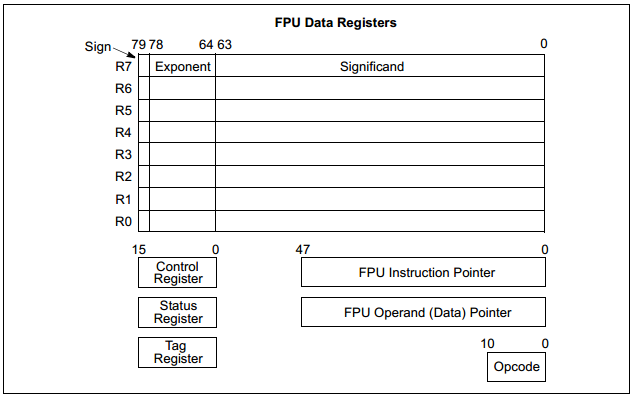
\includegraphics[scale=0.75]{MoiTruongFPU.png}
				\end{center}
				\caption{Môi trường thực thi FPU}				
				\label{fig:MoiTruongFPU}				
			\end{figure}
		\end{center}		
		
	Nếu hoạt động nạp giá trị được thực hiện khi TOP = 0 giá trị mới của TOP được thiết lập là 7. Ngoại lệ ngăn xếp bị tràn trên xảy ra giá trị được nạp không được ghi đè lên thanh ghi.			
			\begin{center}
			\begin{figure}[htp]
				\begin{center}
					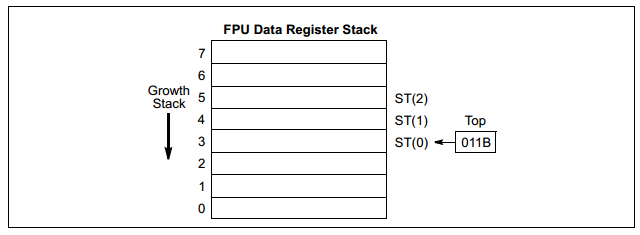
\includegraphics[scale=0.75]{StackFPU.png}
				\end{center}
				\caption{Ngăn xếp thanh ghi dữ liệu FPU}				
				\label{fig:StackFPU}				
			\end{figure}
		\end{center}		
			
			Có nhiều câu lệnh xử lý dấu chấm động cho phép người lập trình thao tác hoàn toàn trên đỉnh stack hoặc thao tác trên các thanh ghi cụ thể mà có quan hệ với đỉnh stack. Assembly hỗ trợ hóa địa chỉ thanh ghi, việc sử dụng thanh ghi ST(0) hoặc đơn giản là ST để biểu diễn thanh ghi hiện tại và ST(i) dùng để biểu diễn thanh ghi thứ i kể từ đỉnh stack (0 $\mathbb{\le}$ i  $\mathbb{\le}$ 7). Ví dụ, nêu đỉnh stack hiện tại là 011B (thanh ghi thứ 3 là đỉnh của stack), khi thực hiện câu lệnh toán học cộng thì nội dung của đỉnh stack sẽ thay đổi theo phép tính cộng hai thanh ghi trong stack ( thanh ghi 3 và 5).
			
	\textit{	FADD ST, ST(2);} \\
	
	Hình ~\ref{fig:VDFPU} cho thấy một ví dụ về cấu trúc ngăn xếp của thanh ghi FPU và câu lệnh thường được sử dụng để thực hiện một phép toán. 
	\begin{itemize}
		\item[1]	Lệnh đầu tiên (FLD value1) tăng thanh ghi con trỏ của stack (hiện tại là đỉnh stack) và nạp giá trị 5.6 từ bộ nhớ vào ST(0). Kết quả của câu lệnh này được chỉ ra ở hình (a).
		\item[2]	Lệnh thứ 2 nhân giá trị trong ST(0) với 2.4 từ bộ nhớ và lưu kết quả vào trong ST(0) như hình (b).
		\item[3] Lệnh thứ 3 tăng đỉnh stack lên và nạp giá trị 3.8 vào ST(0).
		\item[4]	Lệnh thứ 4 nhân giá trị trong ST(0) với 10.3 từ bộ nhớ chính và lưu trữ kết quả trong ST(0) như hình (c).
		\item[5]	Lệnh thứ 5 cộng thêm giá trị của đỉnh stack ST(0) với giá trị trong ST(1) và lưu kết quả vào trong ST(0) như hình (d).
	\end{itemize}
	
		Đây là một ví dụ trong việc thực thi một câu lệnh tính toán xử lý dấu chấm động.
	
	\subsubsection*{Truyền tham số vào stack của thanh ghi FPU}	
	Cũng giống như các thanh ghi xử lý số nguyên, thanh ghi dữ liệu FPU không bị ảnh hưởng bởi các lời gọi thủ tục, hay cách gọi khác, các giá trị được giữ nguyên đến khi có câu lệnh muốn thực thi trên thanh ghi dữ liệu này. Một thủ tục có thể gọi để sử dụng giá trị cho một thủ tục hay câu lệnh khác. Việc gọi thanh ghi bằng cách thông qua con trỏ đỉnh stack hiện tại và cách đặt tên ST(0) và ST(i). Đây là cách gọi thông thường nhất khi muốn lấy giá trị của một thanh ghi trong stack và trả về kết quả trong đỉnh ST(0) khi thực thi câu lệnh hoặc của chương trình.
	
	\begin{center}
			\begin{figure}[htp]
				\begin{center}
					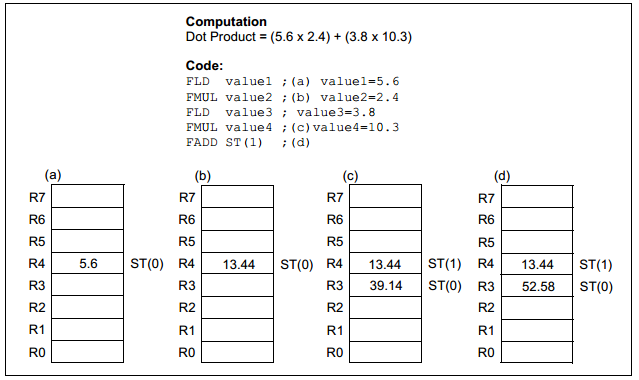
\includegraphics[scale=0.75]{VDFPU.png}
				\end{center}
				\caption{Ví dụ xử lý câu lệnh trong stack của FPU}				
				\label{fig:VDFPU}				
			\end{figure}
		\end{center}	
		
		\newpage
		\subsection*{ Thanh ghi trạng thái FPU}
	Thanh ghi trạng thái FPU 16 bit (hình ~\ref{fig:TrangThaiFPU} ) chỉ ra trạng thái hiện tại của FPU. Bit cờ của thanh ghi trạng thái bao gồm các cờ báo của FPU, con trỏ đỉnh stack, mã điều kiện, cờ báo lỗi, cờ báo lỗi ngoại lệ và cờ báo lỗi stack. FPU thiết lập những bit cờ trong thanh ghi để chỉ ra kết của của phép toán được thực hiện.\\

	Nội dung của thanh ghi trạng thái FPU có thể được lưu vào bộ nhớ bằng cách sử dụng câu lệnh FSTSW/FNSTSW, FSTEN/FNSTENV và FSAVE/FNSAVE. Cũng có thể lưu trữ trong thanh ghi AX của bộ xử lý số nguyên bằng cách sử dụng câu lệnh FSTSW/FNSTSW.\\

		\subsubsection*{Con trỏ đỉnh stack (TOP)}
	Con trỏ trỏ tới thanh ghi dữ liệu hiện tại ở đỉnh stack được chứa trong bit 11 đến 13 của thanh ghi trạng thái FPU. Con trỏ thường được gọi là TOP (đỉnh stack) có giá trị từ 0 đến 7.

		\subsubsection*{ Cờ điều kiện}
	Bốn bit cờ điều kiện của thanh ghi FPU (từ C0 đến C3) chỉ ra kết quả của sự so sánh dấu chấm động và thao tác toán học. Bảng () tóm tắt các loại lệnh mà dấu chấm động sẽ thiết lập bit cờ điều kiện phục vụ cho việc phân loại xử lý ngoại lệ.
	
		\begin{center}
			\begin{figure}[htp]
				\begin{center}
					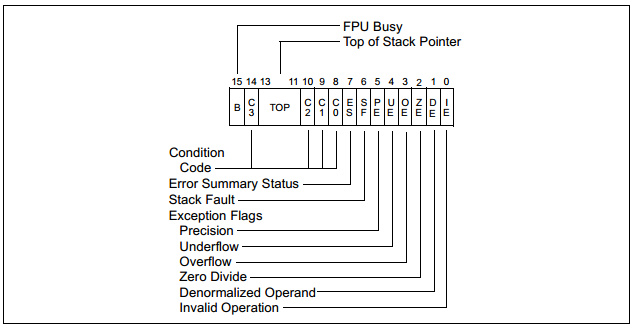
\includegraphics[scale=1]{TrangThaiFPU.png}
				\end{center}
				\caption{Thanh ghi trạng thái FPU}				
				\label{fig:TrangThaiFPU}				
			\end{figure}
		\end{center}	
		
		Như thể hiện trong bảng (), bit cờ điểu kiện C1 được sử dụng trong nhiều câu lệnh. Khi bit cờ IE và SF được bật, để chỉ ra lỗi tràn trên hoặc tràn dưới của stack (IS), bit C1 sẽ giúp phân biệt giữa tràn trên (C1 = 1) và tràn dưới (C1 = 0). Khi bit cờ PE trong thanh ghi trạng thái được bật, để cho thấy kết quả đã được làm tròn, bit C1 sẽ được bật nếu số được làm tròn bằng cách làm tròn lên. Câu lệnh FXAM bật C1 theo bit dấu của giá trị được kiểm tra\\.

	Bit cờ điều kiện C2 được sử dụng bởi câu lệnh FPREM và FPREM1 để thể hiện phép tính khi sử dụng câu lệnh này không thực hiện được. Khi thực hiện được phép tính này, các bit cờ điệu kiện C0, C1 và C3 sẽ được thay đổi theo kết quả của phép tính, dựa vào các bit cuối của kết quả tính được. \\

	Các câu lệnh FPTAN, FSIN, FCOS và FSINCOS bật bit điều kiện C2 khi toán hạng được sử dụng trong câu lệnh này vượt quá phạm vi cho phép từ -263 đến +263. 
	
		\begin{longtable}{ | m{5cm} | m{2cm} |  m{2cm} | m{3cm} | m{2cm}| }
			\hline
				Câu lệnh &  C0 & C1 & C2& C3\\
			\hline
			\hline
				FCOM, FCOMP, FCOMPP, FICOM, FICOMP, FTST, FUCOM, FUCOMP, FUCOMPP & \multicolumn{2}{c|}{Kết quả so sánh} & Không phụ thuộc phép so sánh & 0 hoặc \#IS \\
			\hline
				FCOMI, FCOMP, FUCOMI, FUCOMP	 & \multicolumn{3}{p{7cm}|}{Không thiết lập (Các câu lệnh này thiết lâp cờ EFLAGS) } & \#IS \\
				\hline 
				FAXM & \multicolumn{3}{c|}{Toán hạng} & Bit dấu\\
				\hline 
				FPREM, FPREM1 & Q2 & Q1 & 0=Thực hiện được 1=Không thực hiện được & Q0 hoặc \#IS \\
				\hline
				F2XM1, FADD, FADDP, 	FBSTP, FCMOVcc, FIADD, FDIV, FDIVP, FDIVR, FDIVRP, FIDIV, FIDIVR,	FIMUL, FIST, FISTP, FISUB, FISUBR,FMUL, FMULP, FPATAN, FRNDINT, FSCALE, FST, FSTP, FSUB, FSUBP, FSUBR, FSUBRP,FSQRT, FYL2X, FYL2XP1 & \multicolumn{3}{c|}{Không thiết lập} & Làm tròn hoặc \#IS \\
				\hline
				FCOS, FSIN, FSINCOS, FPTAN & \multicolumn{2}{c|}{Không thiết lập} & 1=Toán hạng nguồn nằm ngoài phạm vi giá trị. & Làm tròn hoặc \#IS(Không thiết lập nếu C2=1) \\
				\hline
				FABS, FBLD, FCHS, FDECSTP, FILD, FINCSTP, FLD, Nạp hằng số, FSTP, FXCH, FXTRACT & \multicolumn{3}{c|}{Không thiết lập} & 0 hoặc \#IS \\
				\hline
				FLDENV, FRSTOR & \multicolumn{4}{c|}{Mỗi bit đươc sao lưu vào trong bộ nhớ}\\
				\hline
				FFREE, FLDCW, FCLEX/FNCLEX, FNOP, FSTCW/FNSTCW, FSTENV/FNSTENV, FSTSW/FNSTSW & \multicolumn{4}{c|}{Không thiết lập}\\
				\hline
				FINIT/FNINIT, FSAVE/FNSAVE & 0 & 0 &0 & 0\\
			\hline
		\end{longtable}	
			
		\subsubsection*{ Cờ ngoại lệ}
	Sáu bit ngoại lệ (bit 0 đến 5) của thanh ghi trạng thái thể hiện một hoặc nhiều trường hợp ngoại lệ xử lý dấu chấm động sẽ được phát hiện từ khi giá trị cuối cùng của bit được chưa bật. (Cờ ngoại lệ sẽ được mô tả trong phần Xử lý ngoại lệ dấu chấm động). \\

	Bit cờ tóm tắt trạng thái ngoại lệ (ES bit 7) được bật khi có bất kỳ cờ ngoại ngoại lệ nào đã được bật. Khi cờ ES được bật, FPU xử lý ngoại lệ được gọi sử dụng phầm mềm sử lý ngoại lệ để xử lý. (Lưu ý, nếu một cờ xử lý ngoại lệ được bật, FPU sẽ vẫn tiếp tục bật những cờ xử lý ngoại lệ nếu có ngoại lệ xảy ra, nhưng cờ ES sẽ vẫn không được bật). \\
	
	Khi cờ ngoại lệ được bật, những cờ được bật sẽ vẫn được bật đến khi cờ được tắt. Để tắt cờ xử lý ngoại lệ có thể xử dụng câu lệnh FCLEX/FNCELX, khởi tạo FPU với câu lệnh FINIT/FNINIT hoặc ghi đè cờ với câu lệnh FRSTOR, FLDENV. \\
		
		B-bit (bit 15) phản ánh nội dung của cờ ES. 
				
		\subsubsection*{ Cờ lỗi stack}
	Cờ báo lỗi stack (bit 6 của thanh ghi trạng thái FPU) thể hiện stack đang bị tràn trên hoặc tràn dưới. FPU bật cờ SF khi phát hiện tràn trên hoặc tràn dưới, nhưng việc bật cờ SF không rõ ràng khi phát hiện một toán hạng không hợp lệ. Khi cờ SF được bật,  cờ điều kiện C1 chỉ ra lỗi: tràn trên (C1 = 1) và tràn dưới (C1 = 0). Khi cờ SF được bật sẽ được giữ nguyên đến khi nào được tắt. Để tắt thi thực thi các câu lệnh FINIT/FNINT, FCLEX/FNCLEX, hoặc FSAVE/FNSAVE).

		\subsection*{ Phân nhánh và sao lưu có điều kiện dựa trên cờ điều kiện FPU}
	Kiến trúc Intel FPU (bắt đầu với các bộ xử lý Pentium Pro) hỗ trợ hai kỹ thuật nhánh và sao lưu có điều kiện theo cách so sánh hai giá trị dấu chấm động. Kỹ thuật được đề cập ở đây là kỹ thuật cũ và kỹ thuật mới.\\
	
	Kỹ thuật cũ có sẵn trong FPU của họ bộ xử lý Pentium. Kỹ thuật này sử dụng các câu lệnh so sánh dấu chấm động (FCOM, FCOMP, FCOMPP, FTST, FUCOMPP, và FICOMP) để so sánh hai giá trị dấu chấm động và thiết lập các cờ điều điện (C0 đến C3) theo kết quả. Nội dung của cờ điều kiện sau đó được sao chép sào cờ trạng thái trong thanh ghi EFLAGS theo hai bước sau (hình ~\ref{fig:SaoLuu}) : 
	\begin{itemize}
		\item[1] Câu lệnh sao lưu FSTSW AX chuyển tranh ghi trạng thái FPU vào trong thanh ghi AX.
		\item[2]	Câu lệnh SAHF sao lưu 8-bit trên của thanh ghi AX, bao gồm cả cờ điều kiện, vào trong 8-bit thấp của thanh ghi cờ EFLAGS. 
	\end{itemize}

	Khi cờ điều kiện đã được sao lưu vào thanh ghi cờ EFLAGS, điều kiện nhảy hoặc điều kiện sao lưu có thể được thực hiện dựa trên các thiết lập mới của cờ trạng thái trong thanh ghi EFLAGS.
	\begin{center}
			\begin{figure}[htp]
				\begin{center}
					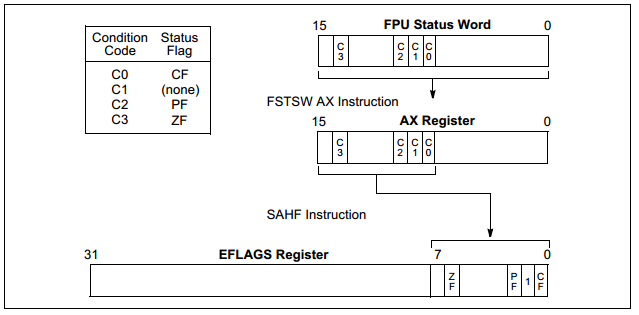
\includegraphics[scale=1]{SaoLuu.png}
				\end{center}
				\caption{Sao lưu có điều kiện}				
				\label{fig:SaoLuu}				
			\end{figure}
		\end{center}	
		
		Kỹ thuật mới chỉ có trong bộ vi xử lý Pentium Pro. Kỹ thuật này sử dụng các câu lệnh () để so sánh hai giá trị dấu dấm dộng và thiết lập cờ ZF, PF và ZF của thanh ghi EFLAGS một cahs trực tiếp. Để thực hiện việc thay đổi này cần một câu lệnh sử dụng kỹ thuật mới, nếu dùng kỹ thuật cũ cần tới ba câu lệnh. \\
		
	Lưu ý rằng các câu lệnh FCMOVcc (chỉ có trong bộ xử lý Pentium Pro) cho phép sao lưu có điều kiện các giá trị dấu chấm động (giá trị này nằm trong thanh ghi dữ liệu FPU) . Để sao lưu có điệu kiện các giá trị dấu chấm động thì những câu lệnh này không xét đến cờ IF.
	
		\subsection*{Thanh ghi điều khiển FPU}
		Thanh ghi điều khiển FPU 16-bit (hình ~\ref{fig:DieuKhienFPU} ) điều khiển độ chính xác của FPU và phương thức làm tròn. Thanh ghi này cũng chứa các bit cờ xử lý ngoại lệ. Nội dung của thanh ghi điều khiển FPU có thể được nạp vào bằng câu lệnh FLDCW và được sao lưu vào bộ nhớ với câu lệnh FSTCW/FNSTCW.\\
		
	Khi FPU được khởi tạo với một trong hai câu lệnh FINIT/FNINIT hoặc FSAVE/FNSAVE, thanh ghi điều khiển FPU tự động thiết lập thông số là 037h, các cờ xử lý ngoại lệ sẽ được bật, cờ làm tròn được thiết lập làm tròn đến số gần nhất, cờ độ chính xác được thiết lập là chính xác kép 64-bits.
		\begin{center}
			\begin{figure}[htp]
				\begin{center}
					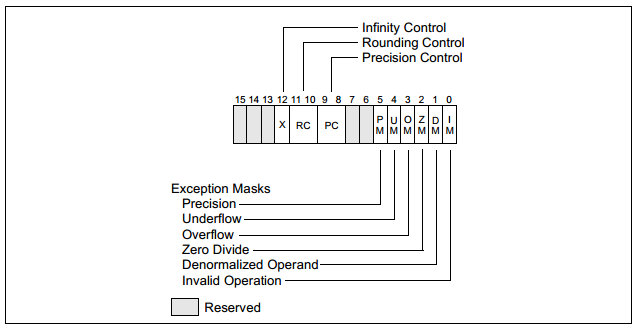
\includegraphics[scale=1]{DieuKhienFPU.png}
				\end{center}
				\caption{Thanh ghi điều khiển FPU}				
				\label{fig:DieuKhienFPU}				
			\end{figure}
		\end{center}	

		\subsubsection*{ Cờ ngoại lệ}
	Cờ ngoại lệ (bit 0 đến bit 5 của thanh ghi điều khiển FPU) có 6 cờ ngoại lệ trong thanh ghi điều khiển FPU giống với 6 cờ ngoại lệ trong thanh ghi trạng thái FPU (bit 0 đến bit 5). Khi một trong các cờ này được bật, tương ứng ngoại lệ của giá trị dấu chấm động sẽ bị chặn khi giá trị được tạo.
.
	\subsubsection*{ Cờ điều khiển độ chính xác}
	Cờ điểu khiển độ chính xác (PC từ bit 8 đến bit 9 của thanh ghi điều khiển FPU) xác định độ chính xác (64, 53 hay 24-bits) của phép tính dấu chấm động được thực hiện bởi FPU (bảng ~\ref{tb:DoChinhXac} ). Mặc định độ chính xác là chính xác mở rộng, sử dụng 64 bits phần định trị làm định dạng cho các thanh ghi giá trị của FPU nhưng cũng có thể thiết lập lại bởi người lập trình, trình biên dịch hoặc hệ điều hành. Thiết lập này phù hợp cho hầu hết các ứng dụng bời vì cho phép các ứng dụng sự thuận tiện và độ chính xác của định dạng chính xác mở rộng.
	\begin{longtable}{|m{6cm}|m{4cm}|}
		\hline
			Độ chính xác & Cờ PC \\
		\hline
		\hline
		Chính xác đơn (24-bits)* & 00B \\
		\hline
		Dành riêng  & 01B \\
		\hline
		Chính xác kép (52-bits)* & 10B \\
		\hline
		Chính xác mở rông (64-bits)* & 11B \\
		\hline	
		\caption{Độ chính xác trong thanh ghi điều khiển FPU}
		\label{tb:DoChinhXac}
	\end{longtable}
	
	Lưu ý: * Các bit đã bao gồm phần bit số nguyên. 
		
	Độ chính xác kép và chính xác đơn được thiết lập sẽ giảm kích thước bit của phần định trị xuống thành 53-bits và 24-bits. Những thiết lập này được cung cấp để hỗ trợ chuẩn IEEE và cho phép tạo lại chính xác kết quả của sự tính toán được thực hiện ở kiểu dữ liệu theo định dạng chính xác thấp hơn. Việc sử dụng độ chính xác thấp hơn, giá trị chính xác bị giảm đi rõ rệt. Khi làm tròn phần định trị không sử dụng những bit bên phải bit 0. \\
	
	Bit điều khiển độ chính xác chỉ ảnh hưởng đến kết của của các câu lệnh xử lý dấu chấm động: FADD, FADDP, FSUB, FSUBP, FSUBR, FSUBRP, FMUL, FUMLP, FDIV, FDIVP, FDIVR, FDIVRP và FSQRT.

		\subsubsection*{Cờ điều khiển làm tròn}
		Cờ điều khiển làm tròn (RC) trong thanh ghi điều khiển FPU (bit 10 và 11) sẽ điều khiển cách kết quả của câu lệnh dấu phẩy động được làm tròn. Có 4 phương thức làm tròn được hỗ trợ (bảng ~\ref{tb:LamTron} ): làm tròn đến số gần nhất, làm tròn lên, làm tròn xuống, làm tròn gần tới 0. Làm tròn đến số gần nhất là phương thức mặc định và phù hợp với hầu hết các ứng dụng, ước lượng được kết quả gần chính xác nhất.
		\begin{longtable}{|m{6cm}|m{2cm}|m{6cm}|}
		\hline
			Phương thức làm tròn & Cờ RC & Mô tả\\
		\hline
		\hline
			Làm tròn đến số gần nhất & 00B & Kết quả được làm tròn là gần nhất với kết quả chính xác.\\
		\hline
			Làm tròn lên (hướng về +$\mathbf{\infty}$) &01B& Kết quả được làm tròn tới số gần nhất, lớn hơn so với kết quả chính xác. \\
		\hline
			Làm tròn xuống (hướng về -$\mathbf{\infty}$) & 10B &Kết quả được làm tròn tới số gần nhất,  nhỏ hơn so với kết quả chính xác. \\
		\hline
			Làm tròn về 0 & 11B & Kết quả được làm tròn tới số gần nhất,  giá trị tuyệt đối của kết quả làm tròn không lớn hơn so với kết quả chính xác\\
		\hline
			\caption{Bảng giá trị  phương thức làm tròn}
			\label{tb:LamTron}
		\end{longtable}
	
		Phương thức làm tròn lên và làm tròn xuống được giới hạn trực tiếp trong lúc làm tròn số và được sử dụng để xác định khoảng giá trị chính xác. Khoảng giá trị được sử dụng để xác định giới hạn trên và giới hạn dưới của kết quả khi thực hiện với nhiều phép tính, khi các kết quả trung gian của phép tính đã được làm tròn số.\\ 
		
	Phương thức làm tròn tới 0 (hay được gọi là “chop”) thường được sử dụng khi thực hiện các phép tính số nguyên trong FPU. \\
	
	Bất cứ khi nào thực hiện các câu lệnh toán học của FPU đưa ra một kết quả chính xác theo định dạng (chính xác đơn, chính xác kép, chính xác mở rộng). Tuy nhiên, thường thì kết quả chính xác của một phép toán hoặc sao lưu không thể mã hóa chính xác theo định dạng của toán hạng.\\
	
	Lấy ví dụ giá trị a có 24 bit phân số. Bit thấp nhất của giá trị a (được gạch chân) không thể mã hóa chính xác theo định dạng chính xác đơn (lúc này chỉ có 23 bit phần phân số).
	
		(a)	$1.0001 0000 1000 0011 1001 0111E_{2} 101$
		
		Để làm tròn kết quả (a), FPU đầu tiên chọn ra hai chuỗi bit có phần phân số gần a nhất (b$\mathbb{\le}$ a $\mathbb{\le}$ c).
		
		(b) $1.0001 0000 1000 0011 1001 011E_{2} 101$
		
		(c)  $1.0001 0000 1000 0011 1001 100E_{2} 101$\\
				
		Sau đó FPU sẽ thiết lập giá trị b và c theo phương thức làm tròn đã được lựa chọn trong cờ RC. Việc làm tròn sẽ tạo ra lỗi trong kết quả mà giá trị được làm tròn nhỉ hơn một đơn vị trong bit cuối của kết quả được làm tròn.\\
		
	Kết quả được làm tròn được gọi là kết quả không chính xác. Khi kết quả không chính xác của câu lệnh FPU được tạo ra, cờ chính xác (PE) trong thanh ghi trạng thái FPU được bật.\\	
	
	Khi cờ xử lý ngoại lệ overflow được bật, kết quả chính xác nằm giữa giá trị cụ thể  và dương vô cực, FPU sẽ làm tròn kết quả theo bảng ~\ref{tb:RCOverflow}.
	\\ \\ \\
		\begin{longtable} {|m{6cm}|m{6cm}|}
			\hline
				Phương thức làm tròn & Kết quả \\			
			\hline						
			\hline
				Làm tròn đến số gần nhất & +$\mathbf{\infty}$\\
			\hline
				Làm tròn về 0 & Giá trị lớn nhất gần nhất mà số thực dương có thể làm tròn.\\
			\hline
				Làm tròn lên (hướng về +$\mathbf{\infty}$) &  +$\mathbf{\infty}$\\
			\hline
				Làm tròn xuống (hướng về -$\mathbf{\infty}$) & Giá trị lớn nhất gần nhất mà số thực dương có thể làm tròn.\\		
			\hline
			\caption{Làm tròn số dương khi overflow xảy ra}
			\label{tb:RCOverflow}
		\end{longtable}

	Khi cờ xử lý ngoại lệ overflow được bật, kết quả chính xác nằm giữa giá trị cụ thể  và âm vô cực, FPU sẽ làm tròn kết quả theo bảng ~\ref{tb:RCUnderflow}
		\begin{longtable} {|m{6cm}|m{6cm}|}
			\hline
				Phương thức làm tròn & Kết quả \\			
			\hline						
			\hline
				Làm tròn đến số gần nhất & -$\mathbf{\infty}$\\
			\hline
				Làm tròn về 0 & Giá trị lớn nhất gần nhất mà số thực âm có thể làm tròn.\\
			\hline
				Làm tròn lên (hướng về +$\mathbf{\infty}$) &  Giá trị lớn nhất gần nhất mà số thực âm có thể làm tròn.\\
			\hline
				Làm tròn xuống (hướng về -$\mathbf{\infty}$) & 	-$\mathbf{\infty}$\\
			\hline			
			\caption{Làm tròn số dương khi Underflow xảy ra}
			\label{tb:RCUnderflow}
		\end{longtable}		
		Phương thức làm tròn không ảnh hưởng đến câu lệnh so sánh, câu lệnh sử dụng kết quả chính xác, hoặc câu lệnh có kết quả là NaN.
		
		\subsection*{Cờ điều khiển vô cùng}
		Cờ điều khiển vô cùng (bit 10 của thanh ghi điều khiển FPU) được cung cấp cho bộ xử lý toán học Intel 281, không có ý nghĩa với bộ xử lý FPU của Pentium Pro hoặc bộ xử lý FPU của Intel 486, hoặc bộ xử lý Intel 387 NPX.
		
		\subsection*{Thẻ FPU}
		Thanh ghi thẻ 16-bit ( hình ~\ref{fig:TagFPU} ) chỉ ra nội dung của 8 thanh ghi dữ liệu FPU (2-bit một biểu diễn cho một thanh ghi). Mỗi thẻ cho biết một thanh ghi chứa một số hợp lệ, bằng không, hoặc một số dấu chấm động đặc biệt (NaN, số vô cùng, denormal, hoặc không hỗ trợ định dạng), hoặc rỗng. Các thẻ FPU được lưu trữ trong FPU trong thanh ghi thẻ FPU. Khi FPU được khởi tạp bằng câu lệnh FINIT/FNINIT hoặc FSAV/FNSAVE, thẻ FPU của mỗi thanh ghi được thiết lập là FFFFh, thể hiện tất cả dữ liệu hiện có trong thanh ghi là rỗng.
		\begin{center}
			\begin{figure}[htp]
				\begin{center}
					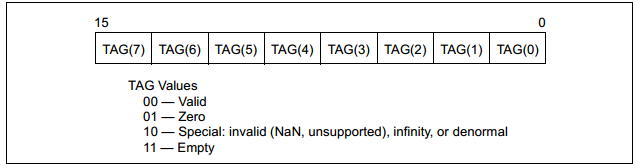
\includegraphics[scale=1]{TagFPU.png}
				\end{center}
				\caption{Thanh ghi điều khiển FPU}				
				\label{fig:TagFPU}				
			\end{figure}
		\end{center}	

	Mỗi thẻ trong thanh ghi thẻ FPU tương ứng với một thanh ghi vật lý (từ 0 đến 7). Đỉnh stack hiện tại (TOP) được lưu trong thanh ghi trạng thái FPU được sử dụng để kết hợp với thanh ghi thẻ liên quan đến ST(0). \\
	
	FPU sử dụng giá trị của thẻ để phát hiện điều kiện tràn trên và tràn dưới của stack. Stack bị tràn trên khi con trỏ TOP giảm đi (do tải dữ liệu vào một thanh ghi hoặc một phép toán được thêm vào) trỏ đến một thanh ghi có giá trị không rỗng. Stack bị tràn dưới khi con trỏ TOP tăng lên (do sao lưu dữ liêu hoặc phép toán lấy dữ liệu ra) trỏ tới một thanh ghi rỗng hoặc thanh ghi rỗng được tham chiếu là một toán hạng. Thanh ghi không rỗng được xác định trong thanh ghi thẻ có chứa nội dung biểu diễn giá trị số 0 (01b), giá trị hợp lệ là (00b), hoặc một giá trị đặc biêt (10b).\\
	
	Các chương trình ứng dụng hoặc xử lý ngoại lệ có thể sử dụng thông tin thẻ để kiểm tra nội dung của thanh ghi dữ liệu FPU mà không cần giải mã dữ liệu của mỗi thanh ghi dữ liệu. Để đọc thanh ghi thẻ, thanh ghi thẻ phải được lưu trong bộ nhớ sử dụng câu lệnh FSTENV/FNSTENV hoặc FSAVE/FNSAVE.  Địa chỉ của thanh ghi thẻ trong bộ nhớ sau khi lưu khi thực hiện một câu lệnh được thể hiện trong hình () đến hình (). \\
	
	Phần mềm không thể trực tiếp tải hoặc sửa đổi giá trị trong thanh ghi thẻ. Câu lệnh FLDENV và FRSTOR tảu một hình ảnh của thanh ghi thẻ vào trong FPU. Tuy nhiên, FPU sử dụng giá trị thanh ghi thẻ để xác định xem các thanh thi dữ liệu là rỗng (11b) hoặc không rỗng (00b, 01b hoặc 10b). Nếu hình ảnh thanh ghi thẻ thể hiện các dữ lệu troang thanh ghi là không rỗng, FPU đọc các giá trị trong thanh ghi dữ liệu và thiết lập thanh ghi thẻ. Hành động này ngăn chẳn một chương trình thiết lập các giá trị trong thanh ghi thẻ biểu diễn không chính xác nội dung hiện tại của thanh ghi dữ liệu.
	
		\subsection*{Con trỏ câu lệnh FPU và con trỏ toán hạng (dữ liệu)}
	Con trỏ lưu trữ trong lệnh FPU và toán hạng (dữ liệu) cho câu lệnh không điều khiển được thực thi trong thanh ghi 48-bit: con trỏ lệnh FPU và con trỏ trỏ tới thanh ghi toán hạng FPU (dữ liệu). (Thông tin được lưu để cung cấp trạng thái thông tin cho xử lý ngoại lệ). 	Con trỏ lưu trữ trong lệnh FPU và thanh ghi con trỏ toán hạng bao gồm một offset (lưu trữ trong bit 0 đến bit 31) và một bộ lọc câu lệnh (lưu trong bits 32 đến 41).\\
	
	Nội dung của câu lệnh FPU và thanh ghi con trỏ toán hạng được giữ nguyên khi có bất kỳ câu lệnh nào của câu lệnh điều khiển (FINIT/FNINIT, FCLEX/FNCLEX, FLDCW, FSTCW/FNSTCW, FSTSW/FNSTSW, FSTENV/FNSTENV, FLDENV, FSAVE/FNSAVE, FRSTOR, và WAIT/FWAIT) được thực thi. Nội dung của thanh ghi toán hạng FPU không xác định được nếu như câu lệnh điều khiển không có bộ nhớ toán hạng.\\
 	
	Những thanh ghi này có thể truy cập bởi các câu lệnh FSTENV/FNSTENV, FLDENV, FINIT/FNINIT, FSAVE/ FNSAVE và FRSTOR. Lệnh FINIT/FNINIT và FSAVE/FNSAVE sẽ xóa nội dung của những thanh ghi này.\\
	
	Tất cả kiến trúc Intel FPU và NPX trừ bộ xử lý 8087, con trỏ lệnh FPU trở tới bất kỳ tiền tố nào mà nó đứng trước câu lệnh. Đối với bộ xử lý 8087, con trỏ lệnh FPU chỉ trỏ tới opcode hiện tại.
	
 		\subsection*{Thanh ghi opcode}
	FPU lưu trữ các opcode của câu lệnh không điều khiển trước khi thực hiện trong thanh ghi opcode 11-bits. (Thông tin này cung cấp trạng thái thông tin cho các xử lý ngoại lệ). Chỉ bytes thứ 1 và 2 của opcode (trước tất cả tiền tố) được lưu trữ trong thanh ghi opcode FPU. Hình () chỉ ra việc mã hóa những byte này.
	
		\subsection*{ Lưu trạng thái FPU}
	Các câu lệnh FSTENV/FNSTENV và FSAVE/FNSAVE lưu các thông tin FPU trong bộ nhớ để sử dụng xử lý ngoại lệ và sử dụng hệ thống khác hay ứng dụng. Câu lệnh FSTENV/FNSTENV lưu nội dung các thanh ghi trạng thái, thanh ghi điều khiển, thanh ghi thẻ, con trỏ lệnh FPU, con trỏ toán hạng FPU và thanh ghi opcode. Câu lệnh FSAVE/FNSAVE lưu thông tin và nội dung của thanh ghi dữ liệu. Lưu ý rằng câu lệnh FSAVE/FNSAVE khởi tạo FPU với các giá trị mặc định (giống như câu lệnh FINIT/FNINIT) sau khi hoàn thành lưu trữ trạng thái của FPU.
	\begin{center}
			\begin{figure}[htp]
				\begin{center}
					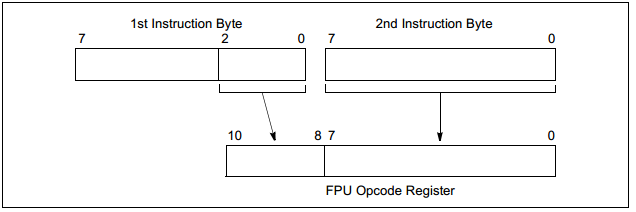
\includegraphics[scale=0.75]{OpcodeFPU.png}
				\end{center}
				\caption{Nội dung thanh ghi opcode FPU}				
				\label{fig:OpFPU}				
			\end{figure}
		\end{center}	

	Cách mà thông tin được lưu trữ trong bộ nhớ phụ thuộc vào chế độ hoạt động của bộ xử lý (chế bộ bảo vệ hoặc chế độ địa chỉ thưc) và kích thước giá trị của toán hạng (32-bit hay 16-bit). Từ hình ()  đến hình (). Trong chế độ virtual-8086 hoặc SMM, địa chỉ thực thể hiện trong hình ().
	\begin{center}
			\begin{figure}[htp]
				\begin{center}
					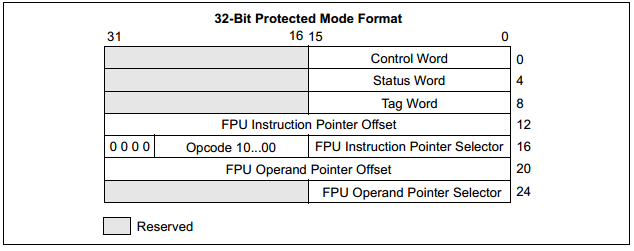
\includegraphics[scale=0.75]{ProtectedFPU.png}
				\end{center}
				\caption{Chế độ bảo vệ (protected) FPU trong bộ nhớ, định dạng 32-bit}				
				\label{fig:ProtectedFPU}				
			\end{figure}
		\end{center}	

		\begin{center}
			\begin{figure}[htp]
				\begin{center}
					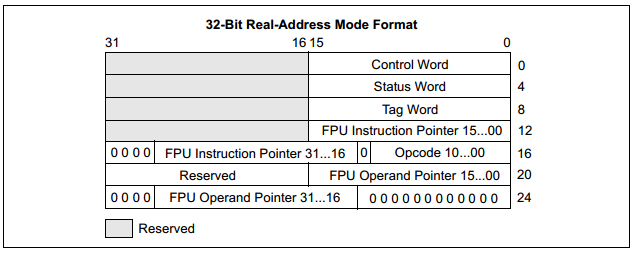
\includegraphics[scale=0.75]{RealFPU.png}
				\end{center}
				\caption{Chế độ địa chỉ thực FPU trong bộ nhớ , định dạng 32-bit}				
				\label{fig:ProtectedFPU}				
			\end{figure}
		\end{center}	
		
		\begin{center}
			\begin{figure}[htp]
				\begin{center}
					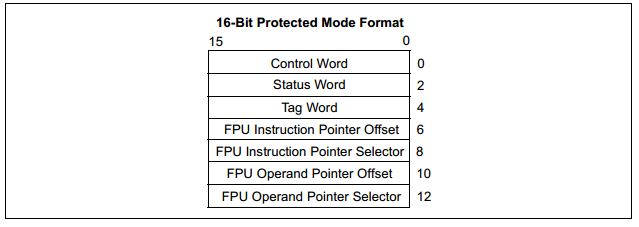
\includegraphics[scale=0.75]{ProtectedFPU16.png}
				\end{center}
				\caption{Chế độ bảo vệ (protected) FPU trong bộ nhớ, định dạng 16-bit}				
				\label{fig:ProtectedFP16U}				
			\end{figure}
		\end{center}	

		\begin{center}
			\begin{figure}[htp]
				\begin{center}
					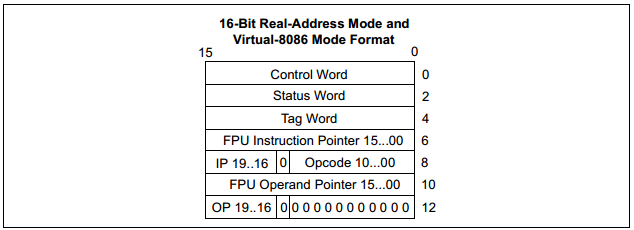
\includegraphics[scale=0.75]{RealFPU16.png}
				\end{center}
				\caption{Chế độ địa chỉ thực FPU trong bộ nhớ , định dạng 16-bit}				
				\label{fig:ProtectedFPU16}				
			\end{figure}
		\end{center}	
		
	Các câu lệnh FLDENV và FRSTOR cho phép thông tin trạng thái FPU được tủa từ bộ nhớ vào FPU. Câu lệnh FLDENV chỉ tải trạng thái, điều khiển, thẻ con trỏ lệnh FPU, con trỏ toán hạng và thanh ghi opcode. Câu eelnhj FRSTOR tải tất cả thanh ghi FPU bao gồm cả thanh ghi dữ liệu.		
		
		\subsubsection{Loại dữ liệu dấu chấm động và định dạng}
		Kiến trúc Intel FPU thao tác trên bảy loại dữ liệu, chia thành ba nhóm: số thực, số nguyên, và số nguyên gói BCD . Hình () cho thấy các định dạng dữ liệu cho mỗi loại dữ liệu FPU. Bảng () cho chiều dài, độ chính xác, và phạm vi bình thường gần đúng có thể được đại diện của từng loại dữ liệu FPU. Giá trị Denormal cũng được hỗ trợ trong mỗi loại thực sự, theo chuẩn của IEEE 854.\\
		
	Với định dạng mở rộng 80-bit biểu diễn ngoại lệ, tất cả các loại dữ liệu chỉ tồn tại trong bộ nhớ. Khi chúng được nạp vào thanh ghi FPU dữ liệu, chúng được chuyển đổi sang định dạng mở rộng-thực và thao tác trên trong định dạng đó.
	\begin{center}
			\begin{figure}[htp]
				\begin{center}
					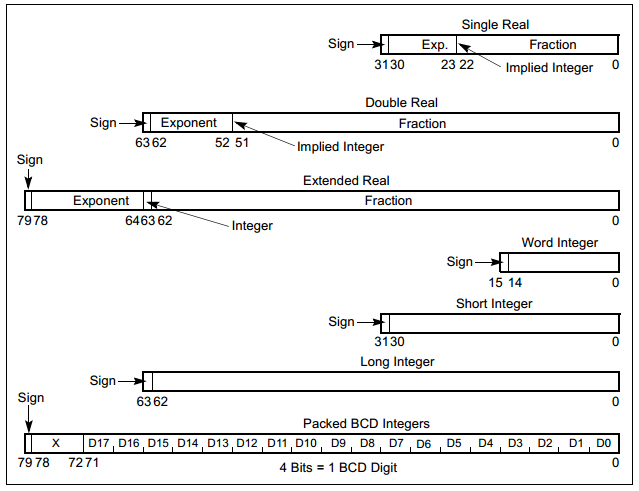
\includegraphics[scale=0.75]{DinhDangFPU.png}
				\end{center}
				\caption{Định dạng loại dữ liệu dấu chấm động}				
				\label{fig:ProtectedFPU16}				
			\end{figure}
		\end{center}	
		
		Khi lưu trữ trong bộ nhớ, byte thấp của một dữ liệu kiểu giá trị FPU được lưu trữ trong địa chỉ đầu tiên chỉ định giá trị đó. Các byte tiếp theo sau đó được lưu trữ trong các địa chỉ cao hơn trong bộ nhớ. Câu lệnh của dấu chấm động nạp và lưu bộ nhớ toán hạng chỉ sử dụng địa chỉ đầu của toán hạng.
		
		\newpage
		\subsection*{Số thực}
		Ba loại dữ liệu số thực của FPU (single-real, double-real, và extended-real) tương ứng với chính xác đơn, đôi chính xác, và định chính xác mở rộng trong các định dạng chuẩn IEEE. Định dạng chính xác mở rộng là định dạng được sử dụng bởi các thanh ghi dữ liệu trong FPU. Bảng () đưa ra độ chính xác và phạm vi của các kiểu dữ liệu và hình () đưa ra các định dạng. Đối với các định dạng single-real và double-real, chỉ có một phần phân số của phần định trị được mã hóa. Số nguyên được giả định là 1 cho tất cả các số trừ 0 và số denormalized hữu hạn. Đối với các định dạng extended-real, các số nguyên được chứa trong bit 63. Ở đây, các số nguyên được thiết lập thành 1 cho số normalized, infinities, và NaNs, và 0 cho số không và số denormalized. \\	 
		
		\newpage
		\begin{longtable}{|l|l|p{2cm}|l|l|}
		 \hline
		 	Kiểu dữ liệu & Độ dài & Chính xác (Bits) & \multicolumn{2}{l|}{Phạm vi giá trị}\\
		 	\cline{4-5}
		 	& & &  Hệ nhị phân & Cơ số 10 \\		
		\hline	
			Binary Real & & & & \\
			Single real &32 &24 & $2^{–126}$ tới $2^{127}$ & 1.18 x $10^{-38}$ tới 3.40 x $10^{38}$\\
			Double real &64 & 53 & $2^{–1022}$ tới 21023 & 2.23 x $10^{–308}  $ tới 1.79 x $10^{308} $\\
			Extended real	&	80 &64&$2^{–16382}  $tới$ 2^{16383} $  & 3.37 x $ 10^{–4932} $ tới 1.18 x $10^{4932}  $\\
		 \hline
		 Binary Integer & & & &\\
			Word integer &16 &15 & $-2 ^{15} $ tới  $ 2^{15} $ -1  &  –32,768   tới 32,767 \\
			Short integer &32 &31 &$ -2^{31} $ tới  $ 2^{31} $  -1 & –2.14 x $10 ^{9 } $ tới 2.14 x $10 ^{9} $\\
			Long integer &64 &63  &$ -2^{63} $ tới  $ 2^{63} $ -1  & -9.22 $ 10^{18} $ tới 9.22  $10 ^{18} $\\
		 \hline					
		 		\caption{Làm tròn số dương khi Underflow xảy ra}
				 \label{tb:DLFPU}
		\end{longtable}
		
		Giải thích 
		Binary Real
		Single real
		Double real 
		Extended real		
		
	Số mũ của từng loại dữ liệu thực được mã hóa ở định dạng cơ bản. Hằng số cơ bản là 127 cho các định dạng single-real, 1023 cho các định dạng doubler-real, và 16.383 cho các định dạng extended-real.\\
	
	Bảng () cho thấy các mã hóa cho tất cả các lớp của các số thực (zero, denormalized-finite, normalized-finite, và vô cùng $\mathbb{\infty}$) và NaNs cho ba loại dữ liệu số thực. Bảng () cũng cung cấp cho các định dạng cho các số thực không xác định.\\

	Khi lưu trữ các giá trị thực sự trong bộ nhớ, giá trị single-real được lưu trữ trong 4 byte liên tiếp trong bộ nhớ, giá trị double-real được lưu trữ trong 8 byte liên tiếp, và các giá trị extended-real được lưu trữ trong 10 byte liên tiếp.\\

	Quy luật chung, giá trị nên được lưu trữ trong bộ nhớ ở định dạng double-real. Định dạng này cung cấp đầy đủ kích thước và độ chính xác để đưa ra kết quả chính xác tối thiểu mà lập trình viên quan tâm. Các định dạng single-real thích hợp cho các ứng dụng bị hạn chế bởi bộ nhớ. Tuy nhiên, single-real cung cấp độ chính xác ít hơn và có thể bị tràn số. Các định dạng single-real hữu ích khi gỡ lỗi các thuật toán, vì làm tròn sẽ thực hiện một cách nhanh chóng ở định dạng này. Các định dạng extended-real thường dành riêng để giữ kết quả trung gian trong các thanh ghi FPU và hằng số. Chiều dài chính xác được thiết kế để đưa ra kết quả cuối cùng từ những phép toán bị ảnh hưởng của làm tròn số và tràn trên hoặc tràn dưới trong các phép tính trung gian. Tuy nhiên, khi một ứng dụng yêu cầu giới hạn chính xác và độ chính xác của các FPU (để lưu trữ dữ liệu, phép toán, và kết quả), các giá trị có thể được lưu trữ trong bộ nhớ ở định dạng mở rộng thực.\\
	
	Các giá trị số thực không xác định là một QNaN được mã hóa và lưu giữ bởi câu lệnh dấu chấm động để đáp ứng với một dấu chấm động không hợp lệ tác ngoại lệ được đánh dấu (xem bảng () ).	
	\newpage
		\begin{longtable}{|l|l|l|l|l|l|}
			\hline
				\multicolumn{2}{|l|}{Loại} & Bit dấu & Bit số mũ & \multicolumn{2}{l|}{Phần định trị} \\
				\cline{5-6}
				\multicolumn{2}{|l|}{} & & & Bit nguyên & Phần thập phân \\
			\hline
				 & +$\mathbb{\infty}$ & 0 & 11..11 & 1 & 00..00 \\
				\cline{2-6}
				  & & 0 & 11..10 & 1 & 11..11 \\
				  & +Normals & . & .& . & . \\
				  & & . & . & . & . \\
				 Số dương & & 0 & 00..01 & 1 & 00..00 \\
				 	\cline{2-6}
				  & & 0 & 00..00 & 0 & 11..11 \\
				  & +Denormals& . & .& . & . \\
				  & & . & . & . & . \\
				  & & 0 & 00..00 & 0 & 00..01 \\
				  \cline{2-6}
				  & +0 & 0& 00..00 & 0 & 00..00 \\
			\hline			
				  & -0 & 1 & 00..00 & 0 & 00..00 \\
				\cline{2-6}
				  & & 1 & 00..00 & 0 & 00..01 \\
				  & -Denormals& . & .& . & . \\
				 Số âm & & . & . & . & . \\
				  & & 1 & 00..00 & 0 & 11..11 \\
				\cline{2-6}
				  & & 1 & 00..01 & 1 & 00..00 \\
				  & -Normals & . & .& . & . \\
				  & & . & . & . & . \\
				  & & 1 & 11..10 & 1 & 11..11 \\
				 \cline{2-6}
				  & -$\mathbb{\infty}$ & 1 & 11..11 & 1 & 00..00 \\
			\hline			
				  & SNaN & X & 11..11 & 1&  0X..$XX_2$ \\
				\cline{2-6}
				 NaN & QNaN & X & 11..11 & 1& 1X..XX\\
				\cline{2-6}
				  & Không định nghĩa &1 & 11..11& 1  &10..00 \\
			\hline
				\multicolumn{3}{r|}{Single-real} & $\leftarrow$ 8 bits $\to $ & & $\leftarrow$ 23 bits $\to $ \\
				\multicolumn{3}{r|}{Double-real} & $\leftarrow$ 11 bits $\to $ & & $\leftarrow$ 53 bits $\to $ \\
				\multicolumn{3}{r|}{Extended-real} & $\leftarrow$ 15 bits $\to $ & & $\leftarrow$ 63 bits $\to $ \\
				\caption{Mã hóa số thực và NaN}
				\label{tb:MaHoaSoThuc}
		\end{longtable}	
	

	LƯU Ý:
	\begin{itemize}
		\item[1] Bit nguyên được ngụ ý và không được lưu trữ cho các định dạng single-real và double-real.
		 \item[2] Phần phân số của SNaN mã hóa phải khác bit 0.
	\end{itemize}

		\subsection*{ Số nguyên được mã hóa nhị phân}
	Có ba loại số nguyên (word, short và long) có định dạng giống hệt nhau, ngoại trừ chiều dài. Bảng () cho độ chính xác và giới hạn của các kiểu dữ liệu và hình () đưa ra các định dạng. Bảng () đưa ra bảng mã của ba loại nguyên dạng nhị phân.
		\begin{longtable}{|l|l|l|l|}
			\hline
				\multicolumn{2}{|l|}{Lớp dữ liệu} & Bit dấu & Độ lớn \\
			\hline
			\hline
					 & Lớn nhất & 0 & 11..11 \\				
					& . & . &. \\
					Số dương& . & . &. \\
					& . & . &. \\
					 & Nhỏ nhất & 0 & 00..01 \\				
			\hline
				\multicolumn{2}{|l|}{Số 0} & 0 &00..00 \\
			\hline
					 & Lớn nhất & 1 & 11..11 \\				
					& . & . &. \\
					Số âm & . & . &. \\
					& . & . &. \\
					 & Nhỏ nhất & 1 & 00..01 \\	
			\hline
				\multicolumn{2}{|l|}{Số không định nghĩa} & 1 &00..00 \\
			\hline
				\multicolumn{2}{l}{} & Word Integer & $\leftarrow$ 15 bits $\to $ \\
				\multicolumn{2}{l}{} & Short Integer & $\leftarrow$ 31 bits $\to $ \\
				\multicolumn{2}{l}{} & Long Integer & $\leftarrow$ 63 bits $\to $ \\
				\caption{Mã hóa nhị phân số nguyên}
				\label{tb:MaHoaSoNguye}
		\end{longtable}	

	Hầu hết các bit phần định trị của mỗi định dạng là bit dấu (0 là số dương và 1 số âm). Giá trị âm được biểu diễn trong chuẩn bù hau. Số 0 được biểu diễn với tất cả các bit (kể cả bit dấu) thiết lập là bit 0. Lưu ý rằng kiểu dữ liệu word-integer của FPU là giống với kiểu dữ liệu word-integer được sử dụng trong bộ xử lý số nguyên và các định dạng short-integer là giống kiểu dữ liệu doubleword-integer.\\
	
	Giá trị word-integer được lưu trữ trong 2 byte liên tiếp trong bộ nhớ; giá trị short-integer được lưu trữ trong 4 byte liên tiếp; và các giá trị long-integer được lưu trữ trong 8 byte liên tiếp. Khi được nạp vào thanh ghi dữ liệu của FPU, tất cả các số nguyên nhị phân là được biểu diễn theo định dạng mở rộng của số thực.\\
	
	Việc mã hóa số nguyên nhị phân 100..00B biểu diễn cho một trong hai ý nghĩa, tùy thuộc vào hoàn cảnh của việc sử dụng nó: 
	\begin{itemize}
		\item[•] Các số âm lớn nhất được hỗ trợ bởi các định dạng (-$2^{15}$, -$2^{31}$, hoặc$ -2^{63}$ ).
		 \item[•] Các nguyên giá trị không xác định.
	\end{itemize}

			Nếu mã hóa này được sử dụng như một toán hạng nguồn (nạp một số nguyên hoặc câu lệnh toán học sử dụng số nguyên), các FPU hiểu nó như là số âm lớn nhất có thể biểu diễn được trong các định dạng được sử dụng. Nếu các FPU kiểm tra một thao tác không hợp lệ khi lưu trữ một giá trị số nguyên trong bộ nhớ với câu lệnh FIST / FISTP và thao tác ngoại lệ được đánh dấu, các FPU lưu trữ số nguyên không xác định đã được mã hóa trong toán hạng đích như một đánh dấu để xử lý ngoại lệ. Trong tình huống mà giá trị gốc với kiểu mã hóa này có thể bị nhập nhằng, cờ toán hạng không hợp lệ có thể được kiểm tra để xem nếu giá trị kết quả đã được đánh dấu xử lý ngoại lệ. \\
	
		Nếu số nguyên không xác định được lưu trữ trong bộ nhớ và sau đó được nạp lại vào một thanh ghi dữ liệu FPU, nó được hiểu là số âm lớn nhất theo định dạng được hỗ trợ.
		
		\subsection*{Số nguyên cơ số 10}
		Số nguyên cơ số 10 được lưu trữ 10-byte theo định dạng gói BCD. Bảng () cho biết độ chính xác và phạm vi của kiểu dữ liệu này và hình() hiển thị định dạng. Trong định dạng này, 9 byte đầu tiên giữ 18 số BCD, 2 số cho mỗi byte. Các chữ số phần định trị được chứa trong nửa-byte thấp từ byte 0 và chữ số nhất có ý nghĩa được chứa ở nửa byte cao từ byte 9. Phần định trị của byte10 chứa bit dấu (0 số dương và 1 số âm). (Bits 0 đến 6 trong byte 10 không quan tâm bit.) Giá trị âm của số nguyên không được lưu trữ ở dạng bù hai; chúng được phân biệt với các số nguyên thập phân dương bởi các bit dấu.\\
		
		Bảng () biểu diễn mã hóa giá trị có thể có trong kiểu dữ liệu số nguyên thập phân.\\
	
		Các định dạng số nguyên thập phân chỉ tồn tại trong bộ nhớ. Khi một số nguyên thập phân được nạp trong một thanh ghi dữ liệu trong FPU, nó sẽ tự động chuyển đổi sang định dạng số thực mở rộng. Tất cả các số nguyên thập phân biểu diễn ở định dạng số thực mở rộng.\\
		
		Việc đóng gói mã hóa sô không xác định số được lưu trữ theo câu lệnh FBSTP một thao tác ngoại lệ sẽ được đánh dấu. Cố gắng nạp giá trị này với câu lệnh FBLD tạo ra một kết quả không xác định.

		\subsection*{Mã hóa theo định dạng Extended-real số không được hỗ trợ}
		Các định dạng extended-real cho phép mã hóa mà không giống với bất kỳ các cách thể hiện trong Bảng (). Bảng () cho thấy các mã hóa không được hỗ trợ. Một số các mã hóa được hỗ trợ bởi bộ xử lý toán học Intel 287. Tuy nhiên, hầu hết trong các bộ xử lý không được hỗ trợ bởi các bộ xử lý toán học Intel 387, hoặc các FPU trong bộ vi xử lý Intel486, Pentium, hay bộ xử lý Pentium Pro. Những mã hóa không còn được hỗ trợ do những thay đổi trong phiên bản cuối cùng của chuẩn IEEE 754 mà loại bỏ các bảng mã.\\
	
		Các loại mã hóa trước đây gọi là pseudo-Nans, pseudo-infinities, và số un-normal không được hỗ trợ. Bộ xử lý toán học Intel 387 và FPU trong bộ vi xử lý Intel486, Pentium, và bộ xử lý  Pentium Pro tạo ra các ngoại lệ và được đánh dấu khi đang gặp phải giống như xử lý toán hạng không hơp lệ.
		\newpage
		\begin{longtable}{|m{2cm}|l|l|l|l|l|l|l|l|}
			\hline
				Lớp dữ liệu & Bit dấu &  & \multicolumn{6}{l|}{Độ lớn} \\
				\cline{4-9}
				& & & Số & Số & Số & Số & .... & Số \\
			\hline
				Số dương lớn & 0 & 0000000 & 1001 & 1001 & 1001 & 1001 & ...  & 1001 \\
			\hline
				& . & . & . & . & . & . & & \\
			\hline
				& . & . & . & . & . & . &  &\\
			\hline
				Số nhỏ & 0 & 0000000  & 0000 & 0000 & 0000 & 0000 & ... & 0001 \\
			\hline
				Số +0 & 0 & 0000000 & 0000 & 0000 & 0000 & 0000 & ... & 0000 \\
			\hline
				Số -0 & 1 & 0000000 & 0000 & 0000 & 0000 & 0000 & ... & 0000 \\
			\hline
				Số nhỏ & 1 & 0000000  & 0000 & 0000 & 0000 & 0000 & ... & 0001 \\
			\hline
				& . & . & . & . & . & . & & \\
			\hline
				& . & . & . & . & . & . &  &\\
			\hline
				Số âm lớn & 1 & 0000000 & 1001 & 1001 & 1001 & 1001 & ...  & 1001 \\
			\hline
				Số không định nghĩa & 1 & 1111111& 1111 & 1111& UUUU* & UUUU & ... &UUUU \\
			\hline
				& \multicolumn{2}{l|}{$\leftarrow$ 1 byte $\to $} & \multicolumn{6}{l|}{$\leftarrow$ 9 byte $\to $}\\
			\hline
				\caption{Mã hóa số nguyên đã được nén (BCD)}
				\label{tb:MaHoaBCD}
		\end{longtable}
		LƯU Ý: * UUUU có nghĩa là giá trị bit không xác định và cũng có thể chứa giá trị bất kỳ.

		\subsubsection{Câu lệnh FPU}				
		Các câu lệnh dấu chấm động được hỗ trợ trong kiến truc Intel FPU có thể được nhóm lại thành sáu loại:
		\begin{itemize}
			\renewcommand{\labelitemi}{\textbullet}
			\item	 Câu lệnh sao lưu dữ liệu
 			\item	Câu lệnh số học cơ bản
			\item	 Câu lệnh so sánh
			\item	 Câu lệnh sử dụng số siêu việt 
			\item	 Câu lệnh nạp dữ liệu.
 			\item	Câu lệnh điều khiển FPU.
		\end{itemize}

	Số siêu việt là là số (thực hoặc phức) nhưng lại không là nghiệm của phương trình đại số nào. Ví dụ: số $\pi $ và \textit{e}. 
	
		
	Phần sau đây mô tả ngắn gọn các câu lệnh trong mỗi loại. 
	\begin{longtable}{|m{2cm}|l|l|l|l|l|}
	\hline
		\multicolumn{2}{|l|}{Lớp dữ liệu} & Bit dấu & Bit mũ & \multicolumn{2}{l|}{Phần định trị}\\
		\cline{5-6}
		 \multicolumn{2}{|l|}{} & & & Bit nguyên & Phần thập phân \\
	\hline
	\hline
		Số thực dương & Số vô cực &0 &  11..11 & 0 & 00..00 \\
		\cline{2-6}
		 &  & 0 &11..10 & 0 & 11..11 \\		
		  &Số không bình thường & . & . & . & . \\
		  &	&0 &00..01& 0&  00..00 \\		 
		 \cline{2-6}
		 & & 0 & 00..00 & 1 & 11..11\\			
		 & Số denormalized  & . & . & . & . \\
		 &	&0 &00..00& 1 &  00..00 \\		
	\hline
		Số thực âm &   & 1 &00..00 & 1 & 11..11 \\		
		 & Số denormalized  & . & . & . & . \\
		 &	& 1  &00..00& 1 &  00..00 \\		
		\cline{2-6}
		 &  &  1 &11..10 & 0 &11..01\\
		  & Số không bình thường  & . & . & . & . \\
		 &	& 1  &00..01 & 0 &  00..00 \\		
		 \cline{2-6}
		 & Số vô cực  & 1 & 11..11 & 0 & 00..00\\
	\hline
		NaN&  & 1  &11..11 & 0 & 01..11 \\
		& Signaling  & . & . & . & . \\
		 &	& 1  &11..11& 0 &  00..01 \\		
	\hline		
		 & & 1 & 11..11 & 0 & 11.11\\
		 &  Quiet  & . & . & . & . \\
		 &	& 1  &11..11& 0 &  10..00 \\		
	\hline
		 \multicolumn{3}{l|}{} & $\leftarrow$15 bits$\to$ & & $\leftarrow$ 63 bits $\to$ \\
		\caption{Mã hóa số không được hỗ trợ  theo định dạng extended-real}
		\label{tb:MaHoaExtended}
	\end{longtable}
	
		\subsection*{ Câu lệnh thoát (ESC)}
	Tất cả các câu lệnh trong câu lệnh của FPU được thiết lập vào một nhóm các lệnh gọi là câu lệnh thoát (ESC). Tất cả các câu lệnh có một định dạng mã thông thường, nhưng một chút khác nhau từ các định dạng được sử dụng bởi các câu lệnh số nguyên và hệ điều hành.
	
		\subsection*{Câu lệnh FPU sử dụng toán hạng}
		Hầu hết các câu lệnh xử lý dấu chấm động cầu một hoặc hai toán hạng, được lưu trữ trong các thanh ghi dữ liệu FPU hoặc trong bộ nhớ. (Không có câu lệnh xử lý dấu chấm động lấy toạn hạng trực tiếp).
		
		\subsection*{ Câu lệnh sao lưu dữ liệu}
		Các câu lệnh sao lưu dữ liệu (xem Bảng ~\ref{tb:CauLenhSaoLuu} ) các bước thực hiệnsau đây:
		\begin{itemize}
			\renewcommand{\labelitemi}{\textbullet}
			\item Nạp toán hạng là số thực, số nguyên, hoặc gói BCD từ bộ nhớ vào thanh ghi ST (0).
			\item Lưu trữ các giá trị trong thanh ghi ST (0)  từ bộ nhớ theo định dạng số thực, số nguyên, hoặc gói BCD.
			\item  Di chuyển các giá trị giữa các thanh ghi trong các thanh ghi dữ liệu FPU.
		\end{itemize}		
		\begin{longtable}{|l|m{4cm}|l|m{3cm}|l|m{3cm}|}
			\hline
				\multicolumn{2}{|l|}{Số thực} & \multicolumn{2}{l|}{Số thực} & \multicolumn{2}{l|}{Gói số nguyên}\\
			\hline
			\hline
				FLD & Nạp số thực &  FILD & Nạp số nguyên &  FBLD & Nạp gói số nguyên  \\
				FST & Lưu số thực & FIST & Lưu số nguyên & & \\ 
				FSTP & Lưu số thực và Pop & FISTP & Lưu số nguyên và Pop & FBSTP  & Lưu gói số nguyên và Pop\\		    
				FXCH & Hoán đổi & & & & \\
				FCMOVcc & Sao chép có điều kiện  & & & &\\
			\hline
				\caption{Câu lệnh sao lưu dữ liệu}
				\label{tb:CauLenhSaoLuu}
		\end{longtable}
	



		Toán hạng thường được lưu trong thanh ghi dữ liệu FPU ở định dạng extended-real (phụ thuộc vào cờ điều khiển chính xác (PC) ở thanh ghi điều khiển). Câu lệnh FLD (nạp số thực) đẩy một toán hạng thực từ bộ nhớ vào đầu stack thanh ghi dữ liệu FPU. Nếu toán hạng là ở định dạng single-real hoặc double-real, FPU sẽ tự động chuyển đổi sang định dạng extended-real. Câu lệnh này cũng có thể được sử dụng để đẩy các giá trị của một thanh ghi dữ liệu FPU lên trên đỉnh của stack thanh ghi.\\
		
		Câu lệnh FILD (nạp số nguyên) chuyển đổi một toán hạng số nguyên trong bộ nhớ sang định dạng extended-real và đẩy giá trị vào đầu stack thanh ghi. Câu lệnh FBLD (nạp gói BCD số nguyên)  thực hiện các hoạt động nạp cùng với một toán hạng gói BCD trong bộ nhớ.\\
		
		Câu lệnh FST (lưu số thực) và FIST (lưu số nguyên) lưu trữ các giá trị trong thanh ghi ST(0) vào trong bộ nhớ trong theo định dạng của bộ nhớ (số thực hoặc số nguyên, tương ứng). Một lần nữa, việc chuyển đổi định dạng được thực hiện tự động.\\
		
		Câu lệnh FSTP (lưu số thực và pop), FISTP (lưu số nguyên và pop), và FBSTP (lưu gói BCD và pop) lưu trữ các giá trị trong thanh ghi ST (0) vào bộ nhớ trong theo định dạng của bộ nhớ (số thực, số nguyên, hoặc gói BCD), sau đó thực hiện pop (lấy dữ liệu ra) khỏi stack thanh ghi. Khi thực hiện pop, thanh ghi ST (0) được đánh dấu trống và con trỏ stack (TOP) trong thanh ghi trạng thái FPU được tăng lên 1. Câu lệnh FSTP cũng có thể được sử dụng để sao chép giá trị và lưu vào trong thanh ghi ST (0) từ thanh ghi FPU [ST (i)].\\
		
		Câu lệnh FXCH (thay đổi nội dung thanh ghi) thay đổi giá trị trong thanh ghi được chọn trong stack [ST (i)] với giá trị trong ST (0).\\
		
		Câu lệnh FCMOVcc (sao chép có điều kiện) sao chép các giá trị trong thanh ghi được chọn trong stack [ST (i)] vào thanh ghi ST (0). Những câu lệnh sao chép các giá trị chỉ khi các điều kiện quy định với một mã điều kiện (cc) được thỏa mãn (xem bảng ~\ref{tb:MoveIns} ). Các điều kiện được thử nghiệm với các câu lệnh FCMOVcc phụ thuộc vào các cờ trạng thái trong thanh ghi EFLAGS.
	\begin{longtable}{|l|l|l|l|}
			\hline
				Câu lệnh & Cờ trạng thái & Mô tả điều kiện \\
			\hline
			\hline
				FCMOVB & CF=1 & Nhỏ hơn \\
				FCMOVNB & CF=0 &  Lớn hơn hoặc bằng\\
				FCMOVE & ZF=1 & Bằng\\
				FCMOVNE & ZF=0 & Không bằng\\
				FCMOVBE & (CF or ZF)=1 & Nhở hơn hoặc bằng\\
				FCMOVNBE & (CF or ZF)=0 & Lớn hơn \\
				FCMOVU & PF=1 &  Không thứ tự \\
				FCMOVNU& PF=0 & Có thứ tự\\
			\hline
				\caption{Câu lệnh sao chép có điều kiện}
				\label{tb:MoveIns}
		\end{longtable}		
		
		Giống như các câu lệnh CMOVcc, các câu lệnh FCMOVcc là hữu ích cho việc tối ưu hóa cờ IF. Các câu lệnh này cũng giúp loại bỏ các trường hợp tự động ngăt hay dừng đột ngột do bộ xử lý gây ra.\\
		
	Lưu ý: Các câu lệnh FCMOVcc có thể không được hỗ trợ trên một số họ bộ vi xử lý Pro Pentium. Phần mềm có thể kiểm tra xem các câu lệnh FCMOVcc có được hỗ trợ bằng cách kiểm tra thông tin của bộ xử lý tính năng với sự câu lệnh CPUID.

		\subsection*{Câu lệnh nạp hằng số}
		Các câu lệnh sau đây thường được sử dụng để nạp hằng số vào đỉnh stack [ST(0)] của thanh ghi dữ liệu FPU [ST (0)]:
		\begin{itemize}
			\renewcommand{\labelitemi}{}
			\item FLDZ Load +0.0
			\item FLD1 Load +1.0
			\item FLDPI Load $\pi$
			\item FLDL2T Load $log_{2}10$
			\item FLDL2E Load $log_{2}e$
			\item FLDLG2 Load $log_{10}2$
			\item FLDLN2 Load $log_{e}2$
		\end{itemize}					

		Các giá trị không đổi biểu diễn theo định dạng extended-real độ chính xác (64 bit) và chính xác đến gần 19 chữ số thập phân. Chúng được lưu trữ theo một định dạng chính xác hơn định dạng extended-real. Khi nạp hằng số, FPU làm tròn số theo cờ làm tròn RC (điều khiển làm tròn) từ thanh ghi điều khiển FPU. 

		\subsection*{Câu lệnh toán học cơ bản}
		Các câu lệnh xử lý dấu chấm động sau đây thực hiện các phép tính cơ bản trên trường số thực. Khi áp dụng, các câu lệnh phù hợp với tiêu chuẩn IEEE 754:
		\begin{itemize}
			\renewcommand{\labelitemi}{}
			\item	 ADD/FADDP Add real
			\item	FIADD Add integer to real
			\item	FSUB/FSUBP Subtract real
			\item	FISUB Subtract integer from real
			\item	FSUBR/FSUBRP Reverse subtract real
			\item	FISUBR Reverse subtract real from integer
			\item	FMUL/FMULP Multiply real
			\item	FIMUL Multiply integer by real
			\item	FDIV/FDIVP Divide real
			\item	FIDIV Divide real by integer
			\item	FDIVR/FDIVRP Reverse divide
			\item	FIDIVR Reverse divide integer by real
			\item	FABS Absolute value
			\item	FCHS Change sign
			\item	FSQRT Square root
			\item	FPREM Partial remainder
			\item	FPREM1 IEEE partial remainder
			\item	FRNDINT Round to integral value
			\item	FXTRACT Extract exponent and significand
		\end{itemize}
		
		\newpage
	Các câu lệnh cộng, trừ, nhân và chia thực hiện trên các loại toán hạng sau đây:
		\begin{itemize}
			\item[•]	Hai giá trị thanh ghi dữ liệu FPU.
			\item[•]   Một giá trị thanh ghi dữ liệu và giá trị thực hay số nguyên trong bộ nhớ.
		\end{itemize}
 
		Phép toán trong bộ nhớ có thể định dạng là single-real, double-real, short-integer, hoặc word-integer. FPU sẽ tự động chuyển đổi sang định dạng extended-real. \\
		
		Câu lệnh phép trừ và phép chia được cung cấp để nâng cao hiệu quả mã hóa. Ví dụ, câu lệnh FSUB trừ giá trị trong một thanh ghi dữ liệu FPU được chọn [ST (i)] từ giá trị trong thanh ghi ST (0); trong khi đó, câu lệnh FSUBR trừ đi giá trị ST(0) từ giá trị trong ST (i). Các kết quả của cả hai hoạt động này được lưu trữ trong thanh ghi ST(0). Những câu lệnh này loại bỏ giá trị không cần thiết giữa đăng ký ST (0) và một thanh ghi FPU khác để thực hiện phép trừ hoặc phép chia.
Các câu lệnh pop của phép cộng, trừ, nhân và chia pop stack thanh ghi dữ liệu FPU sau khi thực hiện các phép toán số học.\\

		Câu lệnh FPREM tính số dư của hai toán hạng theo cách thức được sử dụng bởi bộ xử lý toán học Intel 8087 và Intel 287, câu lệnh FPREM1 tính số dư theo cách thức đặc tả trong IEEE.\\
		
		Câu lệnh FSQRT tính căn bậc hai của toán hạng nguồn.\\
		
		Câu lệnh FRNDINT làm tròn một giá trị số thực thành giá trị số nguyên gần nhất của nó, theo phương thức làm tròn theo cách thức làm tròn được quy định trong cờ RC từ thanh ghi điều khiển FPU. Câu lệnh này thực hiện chức năng tương tự như các câu lệnh FIST / FISTP, ngoại trừ kết quả được lưu trong định dạng số thực.\\
		
		Câu lệnh FABS, FCHS, và FXTRACT thực hiện các phép tính thuận tiện. Câu lệnh FABS tạo ra giá trị tuyệt đối của toán hạng nguồn. Câu lệnh FCHS thay đổi dấu của toán hạng nguồn. Câu lệnh FXTRACT tách các toán hạng nguồn thành số mũ và phần phân số của toán hạng sau đó lưu trữ mỗi giá trị trong thanh ghi ở định dạng số thực.
		
 		\subsection*{Câu lệnh so sánh và phân loại} 
		Các câu lệnh sau đây so sánh và phân loại giá trị số thực:
		\begin{itemize}
			\renewcommand{\labelitemi}{}
			\item	FCOM/FCOMP/FCOMPP Compare real and set FPU condition code flags.
			\item	FUCOM/FUCOMP/FUCOMPP Unordered compare real and set FPU condition code flags.
			\item	FICOM/FICOMP Compare integer and set FPU condition code flags.
			\item	FCOMI/FCOMIP Compare real and set EFLAGS status flags.
			\item	FUCOMI/FUCOMIP Unordered compare real and set EFLAGS status flags.
			\item	FTST Test (compare real with 0.0).
			\item	FXAM Examine.
		\end{itemize}

		So sánh các giá trị số thực sự khác với so sánh các số nguyên bởi vì giá trị thực có bốn (chứ không phải là ba) các mối quan hệ lẫn nhau: nhỏ hơn, bằng, lớn hơn, và không có thứ tự.\\
		
		Các mối quan hệ không có thứ tự là đúng khi có ít nhất một trong hai giá trị được so sánh là NaN hoặc định dạng không xác định. Thêm mối quan hệ này là cần thiết bởi vì, theo định nghĩa, NaNs không phải là số, vì vậy NaNs không thể nhỏ hơn, bằng hoặc lớn hơn trong các mối quan hệ với giá trị số thực khác.\\
		
		Câu lệnh FCOM, FCOMP, và FCOMPP so sánh giá trị trong thanh ghi ST(0) với một toán hạng nguồn số thực và thiết lập các cờ điều kiện (C0, C2, và C3) trong thanh trạng thái FPU theo kết quả (xem Bảng ~\ref{tb:SettingFPU} ). Nếu một điều kiện không có thứ tự được phát hiện (một hoặc cả hai giá trị là NaN hoặc định dạng không xác định), cờ ngoại lệ toán hạng không hợp lệ được bật.\\
		
		Các câu lệnh pop stack thanh ghi dữ liệu FPU được pop một lần hoặc hai lần sau khi hoạt động so sánh thực hiện xong.\\
		
		Câu lệnh FUCOM, FUCOMP, và FUCOMPP thực hiện giống như các câu lệnh FCOM, FCOMP, và FCOMPP. Sự khác biệt duy nhất với các câu lệnh FUCOM, FUCOMP, và FUCOMPP là nếu một điều kiện không có thứ tự được phát hiện bởi một hoặc cả hai toán hạng là một QNaN, cờ ngoại lệ toán hạng không hợp lệ được bật.
		\begin{longtable}{|l|l|l|l|}
			\hline
				Điều liện	& C3 & C2 & C0 \\
			\hline
			\hline
				ST(0) $>$ Toán hạng nguồn & 0 &  0 &  0 \\
			\hline
				ST(0) $<$ Toán hạng nguồn & 0 &  0 &  1 \\
			\hline
				ST(0) $=$ Toán hạng nguồn & 1 &  0 &  0 \\
			\hline
				Không thứ tự & 1 &  1 &  1 \\
			\hline
				\caption{Thiết lập cờ điều kiện FPU theo phép so sánh số thực}
				\label{tb:SettingFPU}
		\end{longtable}	
		
		Câu lệnh FICOM và FICOMP cũng thực hiện giống như các hướng dẫn FCOM và FCOMP, ngoại trừ các toán hạng nguồn là một giá trị số nguyên trong bộ nhớ. Giá trị số nguyên được tự động chuyển đổi thành định dạng extened-real trước khi so sánh. Câu lệnh FICOMP thực hiện pop stack thanh ghi dữ liệu FPU sau khi thực hiện hoạt động so sánh xong.\\
		
		Câu lệnh FTST thực hiện các hoạt động tương tự như câu lệnh FCOM, ngoại trừ các giá trị trong thanh ghi ST (0) luôn luôn được so sánh với giá trị 0.0.
		
		Câu lệnh FCOMI và FCOMIP là câu lệnh mới trong bộ xử lý Intel Pro Pentium. Câu lệnh thực hiện phép so sánh tương tự như hướng dẫn FCOM và FCOMP, ngoại trừ việc câu lệnh thiết lập các cờ trạng thái (ZF, PF và CF) trong thanh ghi EFLAGS để chỉ ra kết quả của phép so sánh (xem Bảng ~\ref{tb:EFLAGS} ) thay vì các cờ điều kiện FPU. Câu lệnh FCOMI và FCOMIP cho phép lệnh rẽ nhánh điều kiện (JCC) được thực hiện trực tiếp từ kết quả so sánh.
		\begin{longtable}{|l|l|l|l|}
			\hline
				Phép so sanh & ZF & PF & CF \\
			\hline
			\hline
					ST(0) $>$ ST(i) & 0 & 0 & 0 \\	
			\hline
					ST(0) $<$ ST(i) & 0 & 0 & 1 \\	
			\hline
					ST(0) $=$ ST(i) & 1 & 0 & 0 \\	
			\hline
					Không thứ tự & 1 & 1 & 1 \\	
			\hline
				\caption{Thiết lập thanh ghi trạng thái EFLAGS theo phép so sánh số thực}
				\label{tb:EFLAGS}
		\end{longtable}	
		
		Câu lệnh FUCOMI và FUCOMIP thực hiện giống như các hướng dẫn FCOMI và FCOMIP, ngoại trừ việc họ không tạo ra một dấu chấm động không hợp lệ tác ngoại lệ nếu điều kiện không có thứ tự là kết quả của một hoặc cả hai toán hạng là một QNaN. Các hướng dẫn FCOMIP và FUCOMIP bật stack FPU đăng ký sau khi hoạt động so sánh.\\
		
		Các hướng dẫn FXAM xác định việc phân loại các giá trị thực sự trong ST (0) đăng ký (có nghĩa là, cho dù giá trị là số không, một số denormal, một số hữu hạn bình thường, $\mathbb{\infty}$ , một NaN, hoặc một định dạng được hỗ trợ) hoặc đăng ký là trống rỗng. Nó đặt FPU mã điều kiện lá cờ để chỉ ra sự phân loại (xem "FXAM-Kiểm tra" trong Chương 3, Instruction Set tham khảo, trong tay các nhà phát triển của Intel Kiến trúc phần mềm, Volume 2). Nó cũng đặt cờ C1 để chỉ ra các dấu hiệu của giá trị.
		
			\subsection{Phân nhánh theo mã điều kiện FPU}
		Bộ xử lý không cung cấp bất kỳ câu lệnh nào đề kiểm soát dòng chảy của chương trình mà các nhánh rẽ được thiết lập từ lá cờ mã điều kiện (C0, C2, và C3) trong thanh ghi trạng thái FPU. Để phân nhánh dựa vào các cờ trạng thái, thanh ghi trạng thái FPU trước tiên phải được sao lưu vào thanh ghi AX bộ xử lý số nguyên. Câu lệnh FSTSW AX (lưu trạng thái) được sử dụng cho mục đích này. Khi mã cờ đã được sao lưu trong thanh ghi AX, câu lệnh Test được sử dụng để kiểm soát rẽ nhánh có điều kiện như sau:
		\begin{itemize}
				\item[1] 	Kiểm tra kết quả không có thứ tự. Sử dụng câu lệnh TEST để so sánh nội dung của thanh ghi AX với hằng số 0400H (xem Bảng ~\ref{tb:CLTest} ). Thao tác này sẽ xóa cờ ZF trong thanh ghi EFLAGS nếu mã cờ điều kiện đánh dấu kết quả là không có thứ tự; ngược lại cờ ZF sẽ được thiết lập. Câu lệnh JNZ sau đó được sử dụng để chuyển giao điều khiển (nếu cần thiết) để câu lệnh xử lý các toán hạng có thứ tự.								
				\item[2]	Câu lệnh kiểm tra so sánh kết quả. Sử dụng các hằng số được đưa ra trong Bảng ~\ref{tb:CLTest} câu lệnh TEST để kiểm tra cho một số nhỏ hơn, bằng hoặc lớn hơn so với kết quả, sau đó sử dụng lệnh rẽ nhánh có điều kiện tương ứng để chuyển điều khiển chương trình tới đoạn mã thích hợp. 
		\end{itemize}
			\newpage
				\begin{longtable}{|l|l|l|}
					\hline
							Điều kiện & Hằng số & Câu lệnh rẽ nhánh \\
					\hline
					\hline
							ST0 $>$ Toán hạng nguồn & 4500H & JZ \\				
					\hline
							ST0 $<$ Toán hạng nguồn & 0100H & JNZ \\		
					\hline
							ST0 $=$ Toán hạng nguồn & 4000H & JNZ \\		
					\hline
							Không thứ tự  & 0400H & JNZ \\		
					\hline
						\caption{Hằng số câu lệnh Test cho lệnh rẽ nhánh}
						\label{tb:CLTest}
				\end{longtable}		
					
			Nếu một chương trình hay hàm đã được kiểm tra cho kết quả QNaN, thì bước tiếp theo không cần kiểm tra kết quả có thứ tự mỗi khi một so sánh được thực hiện.\\
			
		Một số câu lệnh FPU không sử dụng phép so sánh mà cập nhật mã cờ điều kiện trong thanh ghi trạng thái FPU. Để đảm bảo rằng các từ trạng thái không bị thay đổi, lưu trữ giá trị mã cờ ngay khi thực hiện phép toán so sánh.
		
			\subsection*{Câu lệnh lượng giác}
		Các câu lệnh sau đây thực hiện bốn hàm lượng giác thường gặp:
		\begin{itemize}
				\renewcommand{\labelitemi}{}
				\item	FSIN Sine
				\item	FCOS Cosine
				\item	FSINCOS Sine and cosine
				\item	FPTAN Tangent
				\item	FPATAN Arctangent
		\end{itemize}

		Toán hạng của câu lệnh là một hoặc hai thanh ghi đầu của stack thanh ghi FPUvà trả kết quả của mình vào stack. Các toán hạng nguồn phải định dạng góc là radian.\\
		
		Câu lệnh FSINCOS trả kết quả sin và cosin từ giá trị toán hạng nguồn. Câu lệnh hoạt động nhanh hơn so với thực hiện hai câu lệnh FSIN và FCOS liên tiếp.\\
		
		Câu lệnh FPATAN tính toán arctangent của ST(1) chia cho ST(0). Câu lệnh rất hữu ích cho việc chuyển đổi tọa độ vuông góc với tọa độ cực.

	\subsection*{Hằng số pi}
	Khi đối số (toán hạng nguồn) của hàm số lượng giác là giới hạn, các đối số được tự động giảm để thích hợp với $2\pi$ thông qua cơ chế giảm được sử dụng bởi các câu lệnh FPREM và FPREM1. Giá trị nội bộ của $\pi$ mà kiến trúc Intel FPU sử dụng để giảm đối số và tính toán khác như sau:
	
	
		$\pi = 0.f * 2^{2}$
		
		
		Giá trị:
		
		
		f = C90FDAA2 2168C234 C
		
		
		(Giới hạn của phần định trị ở trên là 32 bit).
		
		
		Giá trị  $\pi$ có 66-bit phần phân số, mà trong đó sẽ được thêm 2 bit vào trong phần định trị của một giá trị extended-real. (66 bits không phải là một số chia hết cho 4 để biểu diễn các chữ số thập lục phân, hai số 0 được thêm vào các giá trị để có thể được biểu diễn ở dạng thập lục phân. Như thế, con số ít nhất-đáng thập lục phân (C) là 1100B, khi hai bit cao nhất đại diện cho bit 67 và 68 của phần định trị.).\\
		
		Giá trị $\pi$ đã được lựa chọn để đảm bảo không mất đi phần định trị trong một toán hạng nguồn, cung cấp giá trị toán hạng trong giới hạn giá trị của câu từng câu lệnh.\\
		
		Nếu kết quả của phép tính sử dụng giá trị $\pi$ chính xác từ các câu lệnh FSIN, FCOS, FSINCOS, hoặc FPTAN, 66-bit phần phân số của  $\pi$ nên được sử dụng. Điều này đảm bảo rằng các kết quả phù hợp với các thuật toán. Sử dụng giá trị làm tròn của $\pi$  có thể gây ra thiếu chính xác trong giá trị kết quả, mà nếu được sử dụng trong mốt số phép tính có thể dẫn đến kết quả là thiếu chính xác.\\
		
		Một phương pháp phổ biến để biểu diễn 66-bit phần phân số của   $\pi$ là để tách các giá trị vào hai số (bit cao  $\pi$  và bit thấp  $\pi$ ) mà khi cộng lại với nhau đưa ra giá trị  $\pi$ được hiển thị giống trước đó tương ứng với 66-bit:
		
		
		 $\pi$  = bit cao $\pi$  + bit thap  $\pi$ 


		Ví dụ, hai giá trị sau đây (được đưa ra trong ký hiệu khoa học với các phần trong thập lục phân và số mũ trong số thập phân) đại diện cho 33 bit cao và 33 bit thấp của phần phân số:
		
		
		Bit cao  $\pi$  = 0.C90FDAA20 x $2^{ 2}$


		Bit thấ  $\pi$  = 0.42D184698 x $2^{-31}$


		Những giá trị này được mã hóa theo định dạng double-real chuẩn IEEE như sau:
		
		
		Bit cao  $\pi$  = 400921FB 54400000


		Bit thấp  $\pi$ = 3DE0B461 1A600000
		
		
		(Lưu ý rằng trong các định dạng double-real IEEE, số mũ (1023) và các phần phân số đã được chuẩn hóa.)
		
		Giá trị  $\pi$  cũng có thể được biểu diễn bằng định dạng extended-real.


		Khi sử dụng giá trị  $\pi$ từ hai phần trong một thuật toán, việc tính toán được thực hiện trên từng phần, với các kết quả riêng. Khi tất cả các tính toán đầy đủ, hai kết quả được ghép với nhau để tạo thành kết quả cuối cùng.\\
		
		Sai số của việc tính toán sử dụng số  $\pi$  có thể tránh được, bằng cách áp dụng các hàm lượng giác có đối số trong giới hạn, hoặc bằng cách thực hiện giảm đối số (xuống đến một mức độ ít hơn  $\frac{\pi}{4}$ ).
		
		\subsection*{Phép toán logarit, epsilon và mũ số}
		Các câu lệnh sau đây cung cấp phép toán khác nhau logarit, số mũ, và tỉ lệ:
		\begin{itemize}
			\renewcommand{\labelitemi}{}
			\item		FYL2X Compute log $(y \times log_{2}x$)
			\item		FYL2XP1 Compute$ log_{e} (y \times log_{2}(x + 1))$
			\item		F2XM1 Compute exponential (2x – 1)
			\item		FSCALE Scale
		\end{itemize}

	Câu lệnh FYL2X và FYL2XP1 thực hiện hai phép tính logarit khác nhau. Câu lệnh FYL2X tính log của$ (y \times log_{2}x$) Thao tác này cho phép tính toán sử dụng các phương trình sau đây:
	
	
		$log_{b}x = (1 / log_{2}b) \times log_{2} x$
		
		
		Câu lệnh FYL2XP1 tính toán epsilon log của $(y \times  log_{2}(x + 1))$. Câu lệnh này cung cấp độ chính xác tối ưu cho các giá trị của epsilon ($\epsilon$) được gần 0.
		
		
		Câu lệnh F2XM1 tính hàm mũ (2x - 1). Câu lệnh này có giá trị nguồn trong phạm vi -1.0 đến +1.0.
		
		
		
		Câu lệnh FSCALE mũ số toán hạng nguồn với số mũ là 2.
		
		\subsection*{Câu lệnh điều khiển FPU}
		Các câu lệnh sau đây kiểm soát trạng thái và phương thức hoạt động của FPU. Đồng thời cũng cho phép xem trạng thái của FPU được kiểm tra:
		\begin{itemize}
			\renewcommand{\labelitemi}{}
			\item		FINIT/FNINITInitialize FPU
			\item		FLDCWLoad FPU control word
			\item		FSTCW/FNSTCWStore FPU control word
			\item		FSTSW/FNSTSWStore FPU status word
			\item		 FCLEX/FNCLEXClear FPU exception flags
			\item		FLDENVLoad FPU environment
			\item		FSTENV/FNSTENVStore FPU environment
			\item		FRSTORRestore FPU state
			\item		FSAVE/FNSAVESave FPU state
			\item		FINCSTPIncrement FPU register stack pointer
			\item		FDECSTP giảm con trỏ stack trong stack thanh ghi FPU
			\item		FFREE làm rỗng các thanh ghi dữ liệu FPU
			\item		FNOP Không thao tác
			\item		WAIT / FWAIT kiểm tra và xử lý các trường hợp ngoại lệ khi được đánh dấu.
		\end{itemize}

		Câu lệnh FINIT / FNINIT khởi tạo các thanh ghi FPU giá trị mặc định.\\
		
		Câu lệnh FLDCW nạp giá trị từ thanh ghi điều khiển FPU từ bộ nhớ. Câu lệnh FSTCW / FNSTCW và FSTSW / FNSTSW lưu giá trị của thanh ghi điều khiển, trạng thái FPU tương ứng vào trong bộ nhớ (hoặc câu lệnh FSTSW / FNSTSW lưu trong một thanh ghi trong bộ xử lý số nguyên).\\
		
		Câu lệnh FSTENV / FNSTENV và FSAVE / FNSAVE lưu các giá trị môi trường FPU và trạng thái tương ứng vào trong bộ nhớ. Môi trường FPU bao gồm tất cả các thanh ghi điều khiển và trạng thái của FPU, thanh ghi dữ liệu FPU. (Câu lệnh FSAVE/FNSAVE cũng khởi tạo các FPU giá trị mặc định, như câu lệnh FINIT / FNINIT, sau lưu môi trường của FPU).\\
		
		Câu lệnh FLDENV và FRSTOR nạp môi trường FPU và trạng thái tương ứng từ bộ nhớ vào các FPU. Những câu lệnh này thường được sử dụng khi chuyển đổi để thực hiện một thao tác riêng biệt hoặc phụ thuộc vào ngữ cảnh. Câu lệnh WAIT / FWAIT là câu lệnh đồng bộ hóa. Những câu lệnh kiểm tra tình trạng từ FPU đánh dấu ngoại lệ FPU. Nếu bất kỳ trường hợp ngoại lệ FPU đánh dấu được tìm thấy, chúng được xử lý trước khi thực hiện câu lệnh tiếp theo trong dòng lệnh. Câu lệnh WAIT / FWAIT được để bộ hóa các câu lệnh thực hiện giữa các FPU và bộ xử lý số nguyên. 
		
		\subsection*{ Câu lệnh không được hỗ trợ trong FPU}
		Trong Intel 8087 có câu lệnh FENI và FDISI và trong bộ xử lý toán học Intel 287 có câu lệnh FSETPM không thực hiện trong bộ xử lý toán học Intel 387, hoặc các bộ vi xử lý Intel486, Pentium, hoặc Pentium Pro. Nếu các opcodes được phát hiện trong các dòng lệnh, FPU thực hiện không thực thi cụ thể và có thanh ghi FPU nào bị ảnh hưởng.

		\subsection{Xử lý ngoại lệ dấu chấm động}
		FPU phát hiện sáu loại ngoại lệ trong khi thực hiện những lệnh dấu phẩy động:
		\begin{itemize}
			\renewcommand{\labelitemi}{\textbullet}
			\item Thao tác không hợp lệ (\#I)
				\begin{itemize}
					\item[-] Stack bị tràn trên hoặc tràn dưới (\#IS)
					\item[-] Thao tác số học không hợp lệ (\#IA)
				\end{itemize}
			\item Divide-by-zero (\#Z)			
			\item  Toán hạng denormalized (\#D)
			\item  Tràn trên số học (\#O)
			\item Tràn dưới số học (\#U)
			\item  Kết quả không chính xác (độ chính xác) (\#P)			
		\end{itemize}

Các thuật ngữ của " \# " biểu tượng theo một hoặc hai chữ cái (ví dụ,\#IS) được sử dụng trong câu lệnh để chỉ ra ngoại lệ. Nó chỉ đơn thuần là một cú pháp viết tắt và không liên quan đến việc xử lý.

		\subsection*{Thao tác không hợp lệ}
		Thao tác xử lý dấu chấm động không hợp lệ ứng với hai loại ngoại lệ sau:
		\begin{itemize}
				\renewcommand{\labelitemi}{\textbullet}
				\item Stack bị tràn trên hoặc tràn dưới (\#IS)
					\item Thao tác số học không hợp lệ (\#IA)
		\end{itemize}
		
		Cờ cho trường hợp ngoại lệ này (IE) là bit 0 của thanh ghi trạng thái FPU, và bit (IM) được đánh dấu là 0 từ thanh ghi điều khiển FPU. Cờ phát hiện lỗi (SF) của thanh ghi trạng thái FPU chỉ ra các loại hình hoạt động gây ra những ngoại lệ. Khi cờ SF được thiết lập là 1, một thao tác nào đó đã dẫn đến tràn trên hoặc tràn dưới; khi cờ SF được thiết lập là 0, một lệnh số học có toán hạng không hợp lệ. Lưu ý rằng FPU thiết lập cờ SF khi nó phát hiện một lỗi stack bị tràn trên hoặc tràn dưới, nhưng không rành mạch khi cờ SF phát hiện toán hạng không hợp lệ. Kết quả là, trạng thái của SF có thể là 1 sau một ngoại lệ thao tác số học không hợp lệ, nếu nó không được thiết lập lại từ lần cuối cùng của lỗi stack bị tràn trên hoặc tràn dưới xảy ra.
		
	\subsubsection*{	Stack bị tràn trên hoặc tràn dưới (\#IS)}
		Thanh ghi thẻ FPU theo dõi những nội dung của stack thanh ghi dữ liệu FPU đăng ký. Sau đó sử dụng thông tin này để phát hiện hai loại lỗi khác nhau stack:
		\begin{itemize}
			\renewcommand{\labelitemi}{\textbullet}
			\item Stack bị tràn trên khi một câu lệnh cố gắng ghi một giá trị vào stack thanh ghi dữ liệu FPU khi hiện tại các thanh ghi đã có dữ liệu.
			\item Stack bị tràn dươi khi một lệnh cố gắng đọc một giá trị từ stack thanh ghi dữ liệu FPU mà các thanh ghi của FPU hiện tại không có dữ liệu.
		\end{itemize} 	
	 
		Khi FPU phát hiện stack bị tràn trên hoặc tràn dưới, cờ IE (bit 0) và cờ SF (bit 6) trong thanh ghi trạng thái FPU được thiết lập là 1. Sau đó thiết lập mã điều kiện cờ C1 (bit 9) trong thanh ghi trạng thái  FPU là 1 nếu stack bị tràn trên hoặc được thiết lập là 0 nếu stack bị tràn dưới.\\
		
		Nếu thao tác không hợp lệ được đánh dấu, FPU sau đó trả về giá trị không xác định của số thực, số nguyên, hoặc BCD-integer tới toán hạng, tùy thuộc vào các câu lệnh được thực thi. Giá trị này sẽ ghi đè lên các ghi đích hoặc bộ nhớ mà câu lệnh được thực thi.\\
		
		Nếu thao tác không hợp lệ không được đánh dấu, một phần mềm xử lý ngoại lệ được gọi để xử lý và top-of-stack pointer (TOP), toán hạng nguồn không thay đổi.\\
		
		Stack bị tràn trên khi mà stack thanh ghi FPU đã chứa đủ tám giá trị và chèn thêm giá trị tiếp theo đẩy vào stack. Stack bị tràn dưới ngược với stack bị tràn trên. Khi mà stack thanh ghi FPU không chứa giá trị nào và lấy thêm giá trị từ đỉnh stack trong khi đỉnh stack hiện tại không đanh chứa giá trị.
		
		\subsubsection*{Thao tác số học không hợp lệ (\#IA)}
		FPU có thể phát hiện một loạt các phép tính số học không hợp lệ mà có thể đã được mã hóa trong một chương trình. Các thao tác này thường chỉ ra lỗi lập trình, chẳng hạn như chia $\mathbb{\infty}$ cho $\mathbb{\infty}$. Bảng ~\ref{tb:InvalidAr}  liệt kê các hoạt động số học không hợp lệ mà các FPU phát hiện. Các thao tác không hợp lệ quy định trong chuẩn IEEE 854.\\
		
	Khi các FPU phát hiện một toán hạng số học không hợp lệ, cờ IE (bit 0) trong thanh ghi trạng thái FPU thiết lập là 1. Nếu thao tác không hợp được đeo đánh dấu, các FPU sau đó trả về một giá trị không xác định được gán vào cho toán hạng đích hoặc gán mã điều kiện dấu chấm động, thể hiện trong Bảng ~\ref{tb:InvalidAr} . Nếu thao tác không hợp lệ không được đánh dấu, một phần mềm xử lý ngoại lệ sẽ được gọi và top-of-stack pointer (TOP), toán hạng nguồn vẫn không thay đổi.
		\begin{longtable}{|m{7cm}|m{7cm}|}
			\hline
				Điều kiện & Kết quả trả về\\
			\hline
			\hline
				Bất kỳ thao tác số học trên một toán hạng mà đó là một định dạng không được hỗ trợ. & Toán hạng đích được gán là giá trị không xác định. \\
			\hline
				Bất kỳ thao tác số học là SNaN. & Toán hạng đích được gán là QNaN.\\
			\hline
				Thao tác so sánh và kiểm tra: một hoặc cả hai toán hạng là NaNs. & Thiết lập các cờ điều kiện (C0, C2, và C3) trong thanh ghi trạng thái FPU là 111B (không so sánh). \\
			\hline
				Phép cộng: toán hạng là vô cùng ngược dấu.
				Phép trừ: toán hạng là vô cùng cùng dấu. & Toán hạng đích được gán là giá trị không xác định. \\
			\hline
				Phép nhân: $\mathbb{\infty}  $ nhân với 0; 0 nhân với $\mathbb{\infty}  $. & Toán hạng đích được gán là giá trị không xác định. \\
			\hline
				Phép chia: $\mathbb{\infty}  $ chia cho $\mathbb{\infty}  $ ; 0 chia cho 0. & Toán hạng đích được gán là giá trị không xác định. \\
			\hline
				Phần dư của câu lệnh FPREM, FPREM1: số chia là 0 hoặc số bị chia là  $\mathbb{\infty}  $. &Toán hạng đích được gán là giá trị không xác định và cờ điều kiện C2 được thiết lập 0. \\
			\hline
				Câu lệnh  FCOS, FPTAN, FSIN, FSINCOS: toán nguồn là $\mathbb{\infty}  $. & oán hạng đích được gán là giá trị không xác định và cờ điều kiện C2 được thiết lập 0. \\
			\hline
			FSQRT: toán hạng là số âm (trừ FSQRT (-0) = -0);
			FYL2X: toán hạng là số âm (trừ FYL2X (-0) = -$\mathbb{\infty}  $);
			FYL2XP1: toán hạng nhỏ hơn -1. & Toán hạng đích được gán là giá trị không xác định. \\
			\hline
			FBSTP: thanh ghi rỗng, hoặc toán hạnh là  NaN, $\mathbb{\infty}  $, hay một giá trị không thể được đại diện trong. &  Toán hạng đích lưu BCD số nguyên là giá trị không xác định.\\
			\hline
				FXCH: một hoặc cả hai thanh ghi toán hạng rỗng. &  Toán hạng đích được gán là giá trị không xác định, sau đó thực hiện hoán đổi. \\
			\hline
			Câu lệnh FIST / FISTP khi toán hạng đầu vào $<>$ MAXINT  kích thước của toán hạng đích. & Toán hạng đích được gán giá trị là MAXNEG. \\
			\hline
				\caption{Thao tác số học không hợp lệ và kết quả trả về}
				\label{tb:InvalidAr}
		\end{longtable}
		
	\subsubsection*{Chia một số cho số 0(\#Z)}
		FPU xảy ra ngoại lệ khi một giá trị dấu chấm động chi cho số 0 khi bất cứ câu lệnh nào cố gắng chia một số hữu hạn khác không toán hạng cho 0. Cờ (ZE) cho trường hợp ngoại lệ này là bit 2 của thanh ghi trạng thái FPU, và ZM  bit 2 của thanh ghi điều khiển FPU được thiết lập giá trị. Các câu lệnh FDIV, FDIVP, FDIVR, FDIVRP, FIDIV, và FIDIVR và các câu lệnh khác mà thực hiện phân chia nội bộ (FYL2X và FXTRACT) có thể được đánh dấu cho trường hợp ngoại lệ chia cho số 0. \\
		
		Khi một ngoại lệ chia cho số 0 xảy ra và các cờ ngoại lệ được đánh dấu, FPU bật cờ ZE và trả về các giá trị thể hiện trong Bảng ~\ref{tb:ChiaCho0}. Nếu ngoại lệ chia cho số 0 không được đánh dấu, cờ ZE được bật, một phần mềm xử lý ngoại lệ sẽ được gọi con trỏ topof-stack (TOP), toán hạng nguồn vẫn không thay đổi.
		\begin{longtable}{|m{6cm}|m{8cm}|}
				\hline
					Điều kiện & Kết quả trả về \\
				\hline
				\hline
					Phép chia hoặc phép chia đảo được chia cho 0. & Kết quả là $\mathbb{\infty}$ với dấu là kết quả của phép toán OR của 2 toán hạng. \\
				\hline
					Câu lệnh FYL2X. &  Kết quả là $\mathbb{\infty}$ với dấu ngược với dấu của toán hạng khác 0 được lưu vào toán hạng đích. \\
				\hline
					Câu lệnh FXTRACT. & ST(1) được lưu là -$\mathbb{\infty}$, ST(0) được lưu là 0 với dấu cùng dấu với toán hạng nguồn.\\
				\hline
					\caption{Điều kiện xảy ra ngoại lệ chia cho số 0 và kết quả trả về}					
					\label{tb:ChiaCho0}
		\end{longtable}		
		\newpage
		\subsubsection*{Toán hạng là số denormal (\#D)}
		FPU báo hiệu ngoại lệ toán hạng là số denormal dựa vào điều kiện sau đây:
			\begin{itemize}
			\renewcommand{\labelitemi}{\textbullet}
			\item Nếu một lệnh số học cố gắng để thao tác trên một toán hạng denormal.
			\item  Nếu một thao tác được thực hiện để nạp một giá trị denormal ở định dạng single-real hoặc duoble-real vào một thanh ghi FPU. (Nếu giá trị denormal được nạp ở định dạng extended-real, ngoại lệ toán hạng số học là denormal toán hạng không bị đánh dấu ngoại lệ này.)
			\end{itemize}
 	
		Cờ (DE) cho trường hợp ngoại lệ là bit 1 của thanh ghi trạng thái FPU, và DM là bit 1 của thanh ghi điều khiển FPU được thiết lập giá trị.\\
		
		Khi ngoại lệ toán hạng là số denormal xảy ra và các bit xử lý ngoại lệ này được đánh dấu, FPU bật cờ DE, sau đó thực hiện thao tác theo câu lệnh. Các toán hạng là số denormal ở định dạng single-real hoặc double-real tự động chuyển đổi sang định dạng extended-real để thực hiện phép toán. Thao tác với số denormal sẽ tạo ra kết quả có số rất nhỏ gần bằng 0. Trong thực tế, các thao tác tiếp theo sẽ thực hiện từ kết quả ở định dạng extended-real. Hầu hết các lập trình viên đánh dấu ngoại lệ này để phép tính toán có thể thực hiện, sau đó phân tích kết quả có thực sự chính xác khi đã được tính toán.
Khi ngoại lệ toán hạng là số denormal xảy ra và các bit xử lý ngoại lệ này được đánh dấu , cờ DE được bật và phần mềm xử lý ngoại lệ được gọi top-of-stack pointer (TOP) và toán hạng nguồn vẫn không thay đổi. Khi toán hạng là số denormal đã làm giảm bit phần định trị do mất bit thấp, giá trị này không nên thao tác. Ngoại trừ toán hạng là số denormal là kết quả từ tính toán có thể dùng để thực hiện các phép toán tiếp theo và ngoại lệ này không được đánh dấu.

		\subsection*{Tràn trên số học (\#O)}
		FPU tràn trên số học (\#O) xảy ra bất cứ khi nào kết quả làm tròn một số học vượt quá giá trị hữu hạn lớn nhất theo định dạng số thực của toán hạng đích của câu lệnh. Ví dụ, nếu định dạng của toán hạng đích là extended-real (80 bit), tràn xảy ra khi kết quả được làm tròn nằm ngoài giới hạn của định dạng từ $-1.0 \times 2^{16.384}$ tới $1,0 \times 2^{16.384}$. Tràn số có thể xảy ra trên các phép tính mà kết quả được lưu trữ trong một thanh ghi FPU. Nó cũng có thể xảy ra khi thao tác sao lưu giá trị (câu lệnh FST, FSTP), khi giá trị ở định dạng extended-real trong một thanh ghi dữ liệu được lưu trữ trong bộ nhớ ở định dạng single-real hoặc double-real. Giới hạn ngưỡng tràn cho các định dạng single-real là $-1.0 \times 2^{128}$ tới $1,0 \times 2^{128}$; giới hạn cho các định dạng double-real là $-1.0 \times 2^{1024}$ tới $1.0 \times 2^{1024}$.\\
		
	Ngoại lệ tràn số không thể xảy ra khi các giá trị ở định dạn số nguyên integer hoặc BCD. Thay vào đó, các ngoại lệ giá trị toán hạng không hợp lệ được đánh dấu.\\
	
	Cờ (OE) cho các ngoại lệ số tràn trên ở bit 3 của thanh ghi trạng thái FPU, và cờ OM bit thứ 3 của thanh ghi điều khiển FPU.\\
	
	Khi một ngoại lệ tràn trên số học xảy ra và đánh dấu các cờ xử lý ngoại lệ cho trường hợp này, các FPU bật OE và trả về các giá trị thể hiện trong Bảng ~\ref{tb:NumberOver}. Giá trị trả lại phụ thuộc vào định dạng làm tròn hiện tại của FPU.
		\begin{longtable}{|l|l|l|}
			\hline
				Phương thức làm tròn & Dấu của kết quả   &  Kết quả đã được làm tròn \\
			\hline
			\hline		
				Làm tròn tới số gần nhất & + & +$\mathbb{\infty}$\\
				& - & -$\mathbb{\infty}$\\
			\hline
				Làm tròn tới -$\mathbb{\infty}$ & + & Số dương lớn nhất có thể làm tròn. \\
				& - & - $\mathbb{\infty}$\\
			\hline
				Làm tròn tới +$\mathbb{\infty}$ & + & + $\mathbb{\infty}$. \\
				& - & Số âm lớn nhất có thể làm tròn\\
			\hline
				Làm tròn tới 0 & + & Số dương lớn nhất có thể làm tròn. \\
				& - & Số âm lớn nhất có thể làm tròn\\
			\hline
				\caption{Kết quả khi trán trên số học xảy ra}
				\label{tb:NumberOver}
		\end{longtable}
		\newpage
		Các thao tác mà FPU khi xảy ra tràn trên số học và cờ xử lý tràn trên số học không đánh dâu, phụ thuộc vào các câu lệnh mà kết quả được lưu trong bộ nhớ hoặc trong các stack thanh ghi dữ liệu.\\
		
		Nếu toán hạng đích là một bộ nhớ, cờ OE được bật và phần mềm xử lý ngoại lệ được gọi top-of-stack pointer (TOP), toán hạng nguồn, đích không thay đổi.\\
		
		Nếu toán hạng đích là thanh ghi trong stack, số mũ của kết quả làm tròn được chia cho $2^{24576}$ và kết quả được lưu giữ cùng với phần định trị trong toán hạng đích. Cờ điều kiện bit C1 trong thanh ghit trạng thái FPU (gọi là trong tình huống này "làm tròn lên") được thiết lập nếu phần định trị được làm tròn lên và xóa nếu kết quả đã làm tròn. Sau khi kết quả được lưu trữ, cờ OE được bật và phần mềm xử lý ngoại lệ được gọi.\\
		
	Khi sử dụng câu lệnh FSCALE, tràn trên có thể xảy ra, mà kết quả là quá lớn để được biểu diễn, ngay cả với một số mũ được điều chỉnh. Ở đây, nếu tràn trên xảy ra một lần nữa, kết quả là một $\mathbb{\infty}$ (vô cùng) được lưu vào trong toán hạng đích.	
		\subsection*{Tràn dưới số học (\#U)}
		FPU xảy ra ngoại lệ tràn dưới số học (\#U) bất cứ khi nào kết quả làm tròn của các câu lệnh là một số "rất nhỏ" (có nghĩa là số nhỏ so với bình thường, giá trị hữu hạn nhỏ nhất có thể mà sẽ phù hợp với các định dạng số thực của toán hạng đích ). Ví dụ, nếu định dạng toán hạng đích là extended-real (80 bit), tràn dưới xảy ra khi kết quả được làm tròn xuống trong khoảng giới hạn $-1.0 \times 2^{-16.382}$ tới $1,0 \times 2^{16.382}$. Giống như tràn trên số học, tràn dưới số học có thể xảy ra trên các phép tính mà kết quả được lưu trữ trong thanh ghi dữ liệu FPU. Ngoại lệ này cũng có thể xảy ra khi thực hiện thao tác lưu (câu lệnh FST,FSTP),  một giá trị trong thanh ghi dữ liệu được lưu trữ vào trong bộ nhớ ở định dạng single-real hoặc double-real. Giới hạn tràn dưới của định dạng single-real là$-1.0 \times 2^{-126}$ tới $1,0 \times 2^{126}$; giới hạn tràn dưới của định double-real là $-1.0 \times 2^{-1022}$ tới $1,0 \times 2^{1022}$. (Ngoại lệ tràn dưới số học không có thể xảy ra khi lưu trữ các giá trị trong một định dạng số nguyên hoặc BCD.)\\
		
		Cờ (UE) xử lý ngoại lệ tràn dưới số học ở bit 4 của thanh ghi trạng thái FPU, và bit UM ở bit 4 của thanh ghi điều khiển FPU được thiết lập.\\
		
		Khi một ngoại lệ tràn dưới số học xảy ra và các bit xử lý ngoại lệ này được đánh dấu, kết quà là số denormalizes. Nếu kết quả số denormalized là chính xác, FPU lưu kết quả trong toán hạng đích, mà không cần thiết lập các cờ UE. Nếu kết quả số denormal không chính xác, FPU bật UE, sau đó đi vào để xử lý các điều kiện ngoại lệ kết quả không chính xác.\\
		
		 Điều quan trọng cần lưu ý là nếu trán dưới sô học được đánh dấu, cờ ngoại lệ tràn dưới số học được bật kết quả số denormalized là không chính xác. Nếu kết quả số denormalized là chính xác, không có cờ nào được thiết lập và không có ngoại lệ xảy ra.\\
		 
		Các thao tác mà FPU khi xảy ra tràn dưới số học và cờ xử lý tràn dưới số học không được đánh dấu, phụ thuộc các câu lệnh để lưu trữ các kết quả trong bộ nhớ hoặc trong stack thanh ghi dữ liệu.\\
		
		Nếu toán hạng đích là stack thanh ghi, số mũ kết quả làm tròn là $2^{24576}$ và kết quả được lưu giữ cùng với phần định trị của toán hạng đích. Mã điều kiện bit C1 trong thanh ghi trạng thái FPU được thiết lập nếu phần định trị được làm tròn lên. Sau khi kết quả được lưu, cờ UE bật và một phần mềm xử lý ngoại lệ được gọi.\\
		
		Khi sử dụng câu lệnh FSCALE, tràn dưới  có thể xảy ra, mà kết quả là quá nhỏ để có thể biểu diễn, thậm chí với số mũ đã được điều chỉnh. Ở đây, nếu tràn dưới số học xảy ra một lần nữa, kết quả là 0 được lưu trữ trong toán hạng đích.
			
		\subsubsection*{Kết quả không chính xác (\#P)} 
		Trường hợp ngoại lệ kết quả không chính xác (còn gọi là các ngoại lệ chính xác) xảy ra nếu kết quả của một thao tác được biểu diễn không chính xác theo định dạng toán hạng đích. Ví dụ, tỷ lệ $\frac{1}{3}$ không thể được biểu diễn chính xác ở dạng nhị phân. Ngoại lệ này được hỗ trợ cho các ứng dụng mà cần phải thực hiện số học chính xác số học. Bởi vì kết quả làm tròn là thường phù hợp cho hầu hết các ứng dụng, ngoại lệ này thường được che dấu. Lưu ý rằng các câu lệnh có độ chính xác cao (FSIN, FCOS, FSINCOS, FPTAN, FPATAN, F2XM1, FYL2X, và FYL2XP1) tạo ra kết quả không chính xác.\\
		
		Ngoại lệ kết quả không chính xác sử dụng cờ (PE) là bit 5 của thanh ghi trạng thái FPU, và PM ở bit 5 của thanh ghi điều khiển FPU.\\
		
		Nếu trường hợp ngoại lệ kết quả không chính xác xảy ra vàlỗi tràn trên số học hoặc tràn dưới số học xảy ra đồng thời, FPU bật PE và lưu trữ các kết quả được làm tròn vào toán hạng đích. Chế độ làm tròn hiện tại xác định các phương thức được sử dụng để làm tròn kết quả. Bit C1 trong thanh ghi trạng thái FPU thể hiện kết quả không chính xác đã được làm tròn lên (C1 được bật) hoặc "không làm tròn lên" (C1 tắt ). Trong trường hợp "không làm tròn lên", các bit ít thấp của các kết quả không chính xác được cắt ngắn vì vậy mà kết quả phù hợp theo định dạng toán hạng đích.\\
		
		Nếu trường hợp ngoại lệ kết quả không chính xác, các bit xử lý ngoại lệ này không đánh dấu và tràn trên số học hoặc tràn dưới số học không xảy ra đồng thời, FPU thực hiện các thao tác gọi một hàm xử lý phần mềm ngoại lệ.\\
		
		Nếu ngoại lệ kết quả không chính xác xảy ra kết hợp với tràn trên số học hoặc tràn dưới số học, một trong những hoạt động sau đây được thực hiện:
		\begin{itemize}
			\renewcommand{\labelitemi}{\textbullet}
			\item	Nếu ngoại lệ kết quả không chính xác xảy ra cùng với cờ xử lý tràn trên số học hoặc tràn dưới số học được đánh dấu, cờ OE hoặc UE cờ và cờ PE được bật và kết quả được lưu như mô tả cho các trường hợp ngoại lệ tràn trên hoặc tràn dưới.
			\item  	Nếu ngoại lệ kết quả không chính xác xảy ra cùng với cờ xử lý tràn trên số học hoặc tràn dưới số học không đánh dấu và cúng sử dụng một toán hạng đích, cờ OE hoặc cờ UE và cờ PE được bật, kết quả được lưu dưới dạng mô tả theo ngoại lệ tràn trên số học hoặc ngoại lệ tràn dưới số học, và gọi phầm mềm xử lý ngoại lệ.
			\item  	Nếu ngoại lệ kết quả không chính xác xảy ra cùng với cờ xử lý tràn trên số học hoặc tràn dưới số học không đánh dấu và sử dụng chung toán hạng đích là bộ nhớ, ngoại lệ kết quả không chính xác bỏ qua.
		\end{itemize}
	
			\subsection*{Thứ tự ưu tiên xử lý ngoại lệ}
		Các bộ xử lý xử lý các trường hợp ngoại lệ theo độ ưu tiên được xác định trước. Khi một câu lệnh tạo ra hai hoặc nhiều điều kiện ngoại lệ, các ưu tiên ngoại lệ xử lý kết quả trong các trường hợp ngoại lệ ưu tiên cao hơn được xử lý trước và các trường hợp ngoại lệ có mức ưu tiên thấp bị bỏ qua. Ví dụ, chia SNaN cho số 0 có khả năng có thể báo hiệu một ngoại lệ toán hạng không hợp lệ  (do các toán hạng SNaN) và một ngoại lệ chia cho 0. Ở đây, nếu cả hai trường hợp ngoại lệ được đánh dấu, FPU xử lý các trường hợp ngoại lệ ưu tiên cao hơn (ngoại lệ toán hạng không hợp lệ) trả lại kết quả không xác định cho toán hạng đích. Ví dụ khác, ngoại lệ toán hạng là số denormal hoặc số không chính xác có thể xảy ra đồng thời với ngoại lệ tràn dưới số học hoặc tràn trên số học, với cả hai trường hợp ngoại lệ được xử lý.\\
		
		Ưu tiên xử lý tường hợp ngoại lệ của dấu chấm động như sau:
		\begin{itemize}
			\item[1.] Toán hạng không hợp lệ, chia như sau:
				\begin{itemize}
					\item[a.] Stack tràn dưới.
					\item[b.] Stack trên.
					\item[c.] Toán hạng có định dạng không được hỗ trợ.
					\item[d.] Toán hạng là SNaN.
				\end{itemize}
			\item[2.]		Toán hạng là QNaN. Mặc dù đây không phải là một ngoại lệ, việc xử lý của một toán hạng QNaN được ưu tiên hơn. Ví dụ, toán hạng QNaN chia cho 0 có kết quả là QNaN, không phải là một ngoại lệ zero-chia.
			\item[3.]		 Bất kỳ trường hợp toán hạng không hợp lệ không được đề cập ở trên xử lý trước ngoại lệ chia cho số 0.
			\item[4.]		Toán hạng là số denormal. Nếu ngoại lệ này được đánh dấu, sau đó thực hiện lệnh tiếp theo, và ngoại lệ ưu tiên thấp có thể xảy ra mà không bị ảnh hưởng.
			\item[5.]		Tràn trên số học và tràn dưới số học xử lý trước ngoại lệ kết quả không chính xác
			\item[6.]		Ngoại lệ kết quả không chính xác.
		\end{itemize}

	Toán hoạng không hợp lệ, chia cho số 0, và trường hợp ngoại lệ toán hạng là số denormal được phát hiện trước khi bắt đầu thao tác câu lệnh xử lý dấu chấm động, trong khi tràn trên, tràn dưới, và kết quả không chính xác được phát hiện sau khi đã được tính toán và cho ra kết quả. Khi một ngoại lệ trước thao tác được phát hiện, stack thanh ghi dữ liệu FPU và bộ nhớ chưa được cập nhật và được đánh dấu trước khi thực hiện các câu lệnh, đông thời câu lệnh đó không được thực hiện. Khi một ngoại lệ phát hiện sau khi thực hiện câu lệnh, stack thanh ghi dữ liệu FPU và bộ nhớ có thể được cập nhật với một kết quả (tùy thuộc vào loại ngoại lệ xảy ra).
	
\newpage
\section{Windows API}

	\subsection{Một vài bộ thư viện cần hỗ trợ}

Ở những bước xây dựng đầu của đề tài, cần ưu tiên tiến hành cho những bộ thư viện phổ biến và được dùng rộng rãi trước tiên. Bảng 2 sau đây sẽ mô tả thông tin những bộ thư viện đã được hỗ trợ bởi BE-PUM:


\begin{longtable}{ | m{3cm} | m{12cm} | }
	\hline
Tên & Chức năng\\
	\hline
	\hline
Dịch vụ nền & Cho phép truy cập vào các nguồn tài nguyên cơ bản có sẵn trong hệ thống của Windows. Bao gồm những thứ như hệ thống tập tin, thiết bị, tiến trình (process), luồng (thread), xử lý lỗi (error handing).
Các chức năng này nằm trong tập tin kernel32.dll trên hệ điều hành Windows 32-bit.\\
	\hline
Dịch vụ nâng cao & Cho phép truy cập vào các chức năng bổ sung. Bao gồm những thứ như Windows registry, tắt/khởi động lại hệ thống (hoặc bãi bỏ - abort), bắt đầu/dừng/tạo ra một dịch vụ, quản lý tài khoản người dùng.
Các chức năng này nằm trong tập tin advapi32.dll trên hệ điều hành Windows 32-bit.\\
	\hline
Giao diện người dùng & Cung cấp các chức năng để tạo và quản lý cửa sổ màn hình và hầu hết những điều khiển cơ bản, chẳng hạn như nút và thanh cuộn, nhận chuột và bàn phím, cũng như các chức năng khác liên quan đến phần giao diện đồ họa người dùng của Windows.\\
	\hline
Các chức năng này nằm trong tập tin user32.dll trên hệ điều hành Windows 32-bit.
Windows shell & Cho phép các ứng dụng truy cập các chức năng được cung cấp bởi các shell của hệ điều hành, cũng như thay đổi nó.
Windows shell ở đây được hiểu là những thành phần cấu tạo nên giao diện đồ họa người dùng của hệ điều hành Windows (bao gồm những thứ như: màn hình desktop, thanh làm việc taskbar và các thành phần con trên nó,…).
Các chức năng này nằm trong tập tin shell32.dll trên hệ điều hành Windows 32-bit.\\
	\hline

\caption[Những bộ thư viện được hỗ trợ bởi BE-PUM]{Những bộ thư viện được hỗ trợ bởi BE-PUM}
\label{table:tblwapilib}
\end{longtable}


	\subsection{Trình tự các bước để ứng dụng JNA vào BE-PUM}

Để  tiến hành áp dụng những khả năng mang lại từ JNA và hệ thống BE-PUM, ta cần trải qua những bước sau đây:
\begin{enumerate}
	\item Ánh xạ tương ứng tên thư viện sẽ được gọi
	\item Ánh xạ tên hàm của API và những kiểu dữ liệu sẽ được dùng (bao gồm kiểu dữ liệu trả về và kiểu dữ liệu của các thông số đầu vào) từ ngôn ngữ lập trình C sang Java
	\item Tiến hành lấy giá trị bộ nhớ của các thông số đầu vào có trong BE-PUM
	\item Truyền các giá trị đó vào những kiểu tương ứng đã được ánh xạ trong Java, gọi API và lấy kết quả trả về.
	\item Lưu giá trị nhận được đó về lại bộ nhớ của BE-PUM
\end{enumerate}


	\subsection{Những kiểu dữ liệu và ánh xạ của chúng vào JNA}

Việc ánh xạ kiểu dữ liệu từ ngôn ngữ lập trình C sang Java được hỗ trợ sẵn bởi JNA cho một số kiểu cơ bản thường dùng như sau:\\

\begin{longtable}{ | m{3cm} | m{5cm} | m{5cm} | }
	\hline
STT & Kiểu dữ liệu trong C & Kiểu dữ liệu trong Java\\
	\hline
	\hline
1 & char & byte\\
	\hline
2 & wchar\_t & char\\
	\hline
3 & short & short\\
	\hline
4 & int & int\\
	\hline
5 & int & boolean\\
	\hline
6 & enum & int (thông thường)\\
	\hline
7  & long long, \_\_int64 & long\\
	\hline
8 & float & float\\
	\hline
9 & double & double\\
	\hline
10 & Con trỏ (VD: void*) & \specialcell{Buffer \\ Pointer}\\
	\hline
11 & \specialcell{Con trỏ (VD: void*, char*) \\ Mảng} & <P>[] (mảng của những kiểu nguyên thủy)\\
	\hline
12 & long & NativeLong\\
	\hline
13 & const char* & String\\
	\hline
14 & const wchar\_t* & WString\\
	\hline
15 & char** & String[]\\
	\hline
16 & wchar\_t** & WString[]\\
	\hline
17 & void** & Pointer[]\\
	\hline
18 & \specialcell{struct* \\ struct} & Structure\\
	\hline
19 & union & Union\\
	\hline
20 & struct[] & Structure[]\\
	\hline
21 & void (*FP)() & Callback\\
	\hline
22 & pointer (<T> *) & PointerType\\
	\hline

\caption[Một số ánh xạ kiểu dữ liệu cơ bản]{Một số ánh xạ kiểu dữ liệu cơ bản}
\label{table:tblwapi_type_mapping}
\end{longtable}
%\end{center}

Căn bản việc ánh xạ kiểu dữ liệu trong JNA được đáp ứng bằng việc kích thước dữ liệu được sử dụng giữa hai ngôn ngữ C và Java có kích thước bằng nhau. JNA hỗ trợ cho việc nạp một mảng các kí tự trong C bằng cách cho vào một đối tượng kiểu String.\\
 
Điểm hỗ trợ mạnh trong JNA đó là sử dụng và truy cập con trỏ của C thông qua đối tượng kiểu Pointer, dù rằng đang làm việc trong ngôn ngữ Java. Và nếu muốn lấy giá trị của một vùng nhớ thay vì chỉ một giá trị ô nhớ như Pointer, ta có thể sử dụng đối tượng kiểu Buffer để JNA đưa giá trị vùng nhớ đó vào trong đối tượng.

	\newpage
	\subsection{Dữ liệu kiểu cấu trúc (structure)} \label{sec:structure}

Một trong những lợi thế to lớn nhất mà JNA mang lại đó là nạp dữ liệu kiểu cấu trúc (structure) vào trong C mà ngôn ngữ Java không có. Điều này được hỗ trợ qua việc tạo ra một lớp mới, kế thừa từ lớp Structure của JNA.\\

Để tạo ra chính xác kiểu cấu trúc để nạp vào JNA, ta cũng phải tìm hiểu và nắm rõ các quy tắc xây dựng và làm việc với kiểu cấu trúc trong ngôn ngữ lập trình C.

		\begin{center}
			\begin{figure}[h]
				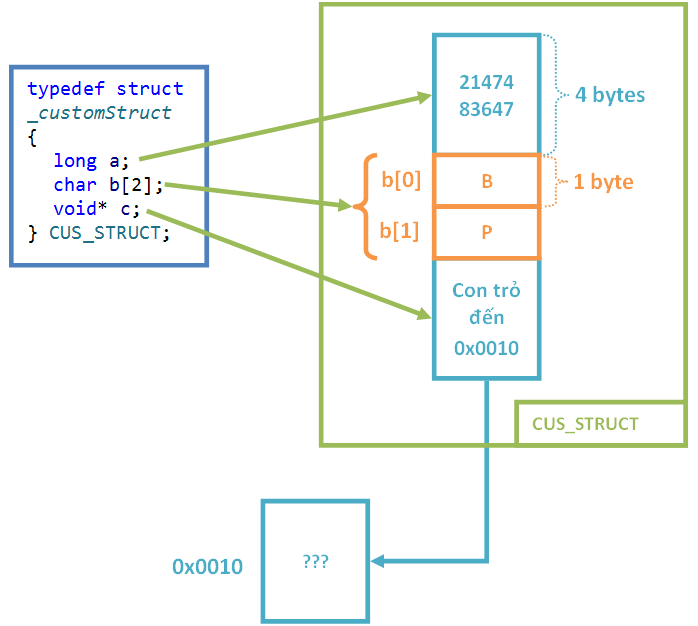
\includegraphics[scale=0.8]{StructureMemoryOrganization.png}
				\caption{Cách sắp xếp và lưu trữ bộ nhớ của structure}				
			\end{figure}
		\end{center}

Một struct trong ngôn ngữ lập trình C là một khai báo dữ liệu kiểu phức hợp, trong đó nó định nghĩa một danh sách các biến được đặt bên trong một khối bộ nhớ. Nó cho phép các biến khác nhau được truy xuất thông qua một con trỏ duy nhất (con trỏ của structure). Một structure có khả năng chứa nhiều kiểu dữ liệu khác nhau từ kiểu dữ liệu nguyên thủy đến kiểu dữ liệu phức tạp khác (enum, structure).\\

Định nghĩa struct khá giống với định nghĩa lớp trong Java, nhưng struct không hề có khả năng khai báo phương thức, cũng như các từ khóa public, private,… như Java. Thêm vào đó, cơ chế cấp phát bộ nhớ của struct chỉ đơn thuần là sự sắp xếp liên tục của các vùng nhớ chứa giá trị của các biến đã được khai báo bên trong. Cách sắp xếp này hoàn toàn tương ứng với ngôn ngữ assembly; do đó ta cần đảm bảo việc lấy ra và gán trở lại bộ nhớ BE-PUM một cách chính xác theo trình tự như vậy.

